\documentclass{article}
\usepackage[utf8]{inputenc}
\usepackage[swedish]{babel}
\usepackage{tocloft}
\usepackage{etoolbox}
\usepackage{graphicx}
\graphicspath{ {images/} }

\usepackage{subcaption}
\usepackage{url}
\usepackage{listings}
%\usepackage{showframe}
%\usepackage[a4paper]{geometry}
\usepackage{fancyhdr}
\usepackage[parfill]{parskip}
\pagestyle{fancy}
\lhead{Grupp 7}

\rhead{\today}
\cfoot{\thepage}

\renewcommand{\contentsname}{Innehåll}

\textheight = 600pt
\footskip = 30pt


\makeatletter
\@addtoreset{section}{part}
\makeatother

\renewcommand\cftpartpresnum{Del~}


\begin{document}
\pagenumbering{roman}

\begin{titlepage}
\begin{center}
  \textbf{\Huge Kandidatarbete}
\end{center}
\begin{center}
  {\Large Redaktör: Pål Kastman}
\end{center}
\begin{center}
  {\Large Datum: 2015-04-20}
\end{center}
\begin{center}
  {\Large \textbf{Version 0.2}}
\end{center}
\end{titlepage}
\newpage
\begin{flushleft}
  {\Large \textbf{Dokumenthistorik}}\\[0.5ex]
  \begin{center}
    \begin{tabular}{ | l | l | p{5cm} | l |}
    \hline
    \textbf{Datum} & \textbf{Version} & \textbf{Utförda ändringar} & \textbf{Utförda av} \\ \hline
    2015-03-13 & 0.1 & Första utkast av gemensam och individuella rapporter & Pål Kastman \\ \hline
    2015-04-20 & 0.2 & Andra utkastet av gemensam och individuella rapporter & Alla \\ \hline
    2015-05-13 & 0.3 & Tredje utkastet av gemensam och individuella rapporter & Alla \\ \hline
    \end{tabular}
  \end{center}
\end{flushleft}

\hfill

\begin{flushleft}
  {\Large \textbf{Projektidentitet}}\\[0.5ex]
  {\small} Detta dokument gäller för grupp 7  i kursen TDDD77 på Linköpings universitet
  \begin{center}
    \begin{tabular}{ | l | l | p{5cm} | l |}
    \hline
    \textbf{Namn} & \textbf{Ansvarsområde} & \textbf{E-post} \\ \hline
    Daniel Rapp & Teamledare & danth407@student.liu.se \\ \hline
    Daniel Falk & Analysansvarig & danfa519@student.liu.se \\ \hline
    Jonas Andersson & Arkitekt & jonan111@student.liu.se \\ \hline
    Albert Karlsson & Kvalitetssamordnare & albka735@student.liu.se \\ \hline
    Erik Malmberg & Testledare & erima694@student.liu.se \\ \hline
    Pål Kastman & Dokumentansvarig & palka285@student.liu.se \\ \hline
    \end{tabular}
\end{center}
\end{flushleft}

\begin{flushleft}
\textbf{Kund} \\ Region Östergötland \\
\end{flushleft}
\begin{flushleft}
\textbf{Kundkontakt} \\ 
Daniel Hall, daniel.hall@regionostergotland.se \\
Erik Sundvall, erik.sundvall@regionostergotland.se \\
Ingrid Hallander, ingrid.hallander@regionostergotland.se \\
\end{flushleft}
\begin{flushleft}
\textbf{Handledare} \\ Lena Buffoni, lena.buffoni@liu.se \\
\end{flushleft}
\begin{flushleft}
\textbf{Handledare} \\ Kristian Sandahl, kristian.sandahl@liu.se \\
\end{flushleft}

\newpage
\tableofcontents
\newpage
\pagenumbering{arabic}

\part{Gemensamma erfarenheter och diskussion}

\section{Inledning}
Detta avsnitt behandlar varför detta projekt utförs.
\subsection{Motivering}

Region Östergötland har idag ett system med handböcker som en sjuksköterska går igenom inför varje operation. I dessa handböcker finns bland annat förberedelse-uppgifter och plocklistor. Handböckerna är idag inte interaktiva på något sätt, istället skrivs plocklistan och förberedelse\-uppgifterna ut och bockas av för hand. Plattformen med handböcker kan heller inte återanvändas på olika avdelningar på grund utav licensproblem. Utöver detta system så finns ett annat separat system, som heter kartoteket, för uppgifter om vilka artiklar som finns och var i lagret de ligger. Detta gör att personalen som ska förbereda inför operationer behöver gå in i två olika system om de inte vet var alla artiklar ligger.\\*

\subsection{Syfte}
Uppgiften som gruppen har fått är att skapa ett nytt system med handböcker som har interaktiva förberedelse-och plocklistor. Listorna ska uppdateras kontinuerligt när de bockas av så flera personer kan jobba på dem samtidigt. Plocklistan ska också innehålla uppgifter om var artiklarna ligger. Tanken är att personalen 
ska använda en iPad för listorna så de kan gå runt och plocka i lagret och bocka av samtidigt. \\*
I mån av tid ska också extra funktionalitet implementeras. Till exempel sortera plocklistan med avseende på närmsta väg mellan artiklarna, lagersaldo och media i handböckerna. \\*
Hela systemet ska ligga under en open-source licens så det kan användas fritt av alla.    
\subsection{Frågeställning}
Rapporten ska besvara följande frågeställningar.
\begin{itemize}
\item Hur kan ett system för operationsförberedelser realiseras så arbetet blir lättare och mer effektivt?
\item Vilka strategier kan användas för effektiv utveckling i en grupp där kunskapsnivån varierar? 
\end{itemize}

\subsection{Avgränsningar}
Den här rapporten beskriver hur ett system för operationsförberedelser på universitetssjukhuset i Linköping kan realiseras. Andra sjukhus kan ha andra rutiner vilket får konsekvensen att systemet inte fungerar där.

Kunden ville också att ett lagersaldo i systemet skulle integreras och göra det möjligt att skanna av artiklar då dessa plockas. Vidare ville kunden även att systemet skulle ge möjlighet att välja mellan olika kliniker i regionen. Tiden kändes inte tillräckligt för att åstadkomma dessa implementeringar därför klargjordes det i ett tidigt skede att få bra grundläggande funktionalitet hade högre prioritet än dessa funktioner. En kompromiss gjordes där dessa krav fick prioritet 2 vilket innebar att kraven var önskvärda och skulle implementeras i mån av tid, eller prioritet 3 där kraven sågs som en framtida utbyggnad.

Hur man ska jobba i projektgrupper med olika kunskapsnivåer tas fram genom undersökningar i projektgrupp 7 i kursen TDDC77 på Linköpings Universitet. Resultaten av denna undersökning kan kanske därför inte appliceras i situationer som inte kan likställas med situationen i projektgruppen.

\section{Bakgrund}
Studenterna som studerar kursen TDDD77 fick i januari 2015 ett uppdrag att utföra ett kandidatarbete. Först fick gruppen rangordna flera projektdirektiv för att sedan få ett av dessa uppdrag tilldelat sig. Grupp 7 fick då projektet operationsförberedelser som skickades in av Region Östergötland.

\subsection{Programspråk och bibliotek}
I detta projekt kommer följande programspråk och bibliotek att användas.

\subsubsection{Node.js}
Node.js är en plattform för att skapa applikationer till framförallt webbservrar. Det finns en inbyggd pakethanterare vid namn npm som gör det enkelt att inkludera både små och stora bibliotek i sina projekt. Det är därför väldigt enkelt att använda sig av ett bibliotek istället för att skriva all funktionalitet själv.

\subsubsection{Keystone.js}
Keystone.js är ett så kallat ''content management system'' som bland annat innehåller ett kraftfullt administrationsverktyg och en databashanterare.

\subsubsection{Socket.IO}
Socket.IO är en modul till Node.js. Socket.IO använder sig av websockets för att kommunicera mellan front-end och back-end. Med hjälp av Socket.IO så kan man skicka data från en klient till alla andra anslutna klienter och visa datan som skickades utan att någon sida behöver laddas om.
Socket.IO har olika komponenter för front-end och back-end. Händelser som skickas från den ena sidan hanteras av motsvarande händelsehanterare på den andra sidan. Varje händelse identifieras med hjälp av en sträng. Det finns några färdiga händelser i Socket.IO exempelvis händelsen "connection" på serversidan fås då en klient har anslutit till Socket.IO.

\subsubsection{MongoDB}
MongoDB är en NoSql dokumentbaserad databas som stödjer stödjer många olika plattformar.

\subsubsection{Handlebars}
Handlebars är ett så kallat ''template language'' som är byggt från Mustache. Handlebars ger bland annat möjlighet till att lägga in mindre logik i html kod samt att från html filer komma åt variabler som finns definierade i javascript filer.

\subsubsection{REST}

\subsubsection{Wkhtmltopdf}
Wkhtmltopdf är ett program som tar en hemsida eller en html-fil och skapar en pdf av den. Programmet har många olika parametrar som kan ändras t.ex. mediatyp så pdf-filen kan se ut som en utskrift av hemsidan. För att kunna använda detta programmet med Node.js finns det också en Node.js-modul med samma namn som skickar kommandon till programmet.


\section{Teori}
För att kunna svara på frågeställningar så måste några begrepp i dem defineras.
Effektivt defineras i detta fallet som att det tar kortare tid för operationsförberedelser och kräver mindre av personalen, till exempel att personalen inte ska behöva hålla lika mycket inforamation i huvudet. 
Lättare defineras som att det går snabbare för nyanställda, och personer som tillfälligt är på en avdelning de inte brukar jobba på, att lära sig rutinerna och kunna utföra arbetet.

Effektiviseringen av sjukvården och hur den ska ske är frågor som diskuterats flitigt de senaste åren. Region Östergötland har gjort tester för att kontrollera hur en operationsförberedelse kan effektiviseras. Ett av dessa tester gick ut på att undersöka hur lång tid det tar att plocka lagerartiklar då information om lagerplats finns lättillängligt gentemot hur lång tid det tar med nuvarande system. Resultatet av detta var att det tog 5 minuter för en person att plocka materialet då lagerplats fanns tillgängligt och 30 minuter för en sjuksköterska med lång erfarenhet med nuvarande system \cite{Elisabeth}. Detta visar att det finns stora tidsvinster i att bygga ett system som underlättar operationsförberedelser.

\subsection{Säkerhetskopiering och reservsystem}
Det ställs stora krav på att handböckerna alltid ska finnas tillgängliga då de ska användas på ett sjukhus där ett fel kan få stora konsekvenser. Detta innebär att ett reservsystem måste finnas till hands ifall systemet slutar fungera. Detta har lösts genom ett system där pdf-kopior av handböcker skapas. Handböckerna hamnar i en mapp-struktur där de sorteras på specialitet och operation. Kopian sparas med ett versionnummer, vilket gör att kopior av gamla versioner av operationer fortfarande finns kvar och kan skrivas ut. Var denna mapp-strukturen ska hamna bestäms i en konfigurationsfil.
Kopiorna skapas genom att en funktion, som kollar igenom alla handböcker för att se om har uppdaterats sedan senaste kopieringen, körs med ett givet tidsintervall som ställs in i konfigurationsfilen. Om en operation har uppdaterats så körs en funktion som använder en modul, som heter wkhtmltopdf, för att kalla på ett program som också heter wkhtmltopdf. Wkhtmltopdf använder en osynlig webbläsare för att skapa en pdf-kopia. Hur kopiorna ser ut kan ses i figur \ref{fig:pdf-start} och figur \ref{fig:pdf-end}. Utseendet ändras genom att speciell css för utskrift finns och wkhtmltopdf körs med utskrift som mediatyp. 
Det finns också ett REST-api för att skapa pdf-kopior. Detta används dock inte någonstans. Men en vidareutveckling på detta vore att implementera att en ny pdf-kopia skapas så fort en operation har uppdaterats. 

\textbf{KOMMENTAR FRÅN RAPP}: Jag kommenterade bort denna bild
därför att den inte finns i \textit{images/}, vilket
ledde till att det inte gick att kompilera \textit{kandidatarbete.tex}.
(Samma för \textit{pdf-end.png} nedan.) Kanske glömde du \textit{git add .}?
%\begin{figure}
%  \centering
%  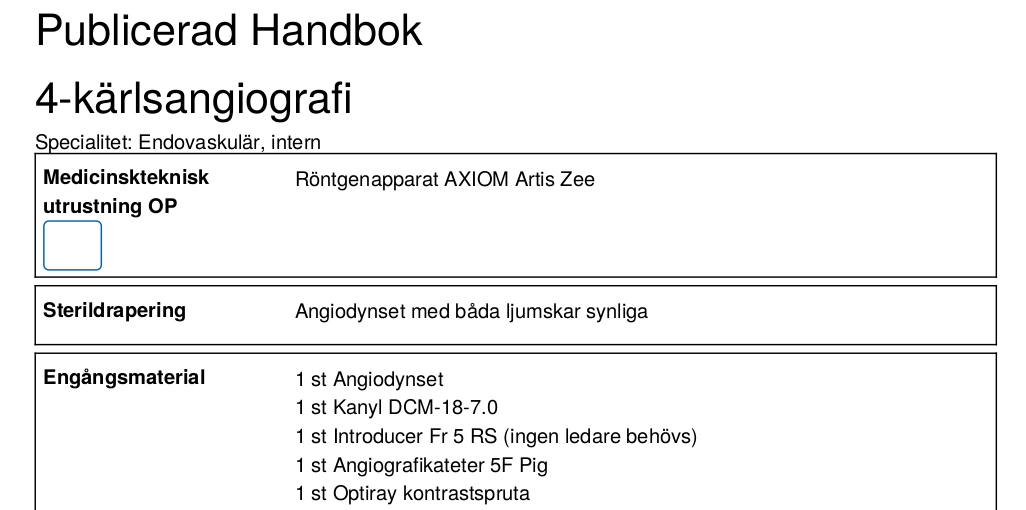
\includegraphics[width=0.9\textwidth]{images/pdf-start.png}
%  \caption{Början på en pdf-kopia.}
%  \label{fig:pdf-start}
%\end{figure}

%\begin{figure}
%  \centering
%  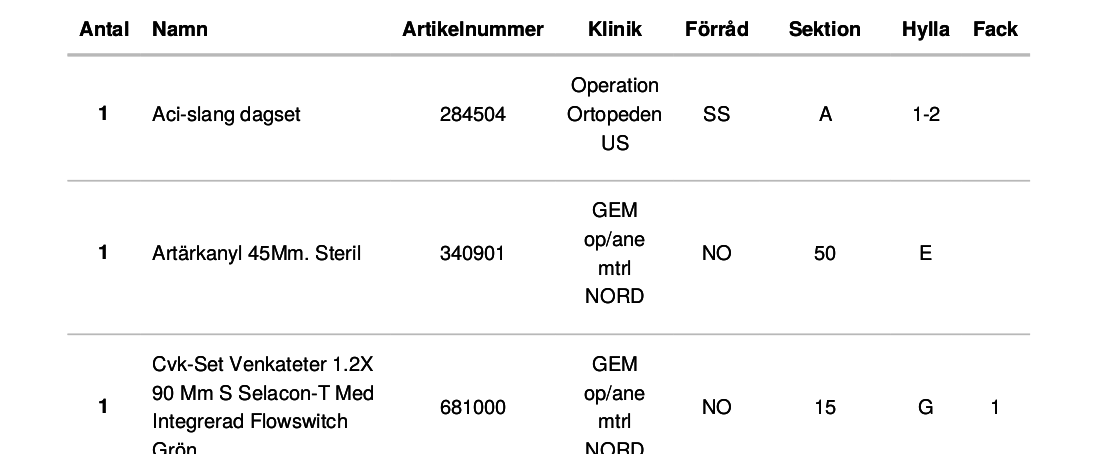
\includegraphics[width=0.9\textwidth]{images/pdf-end.png}
%  \caption{Plocklista i en pdf-kopia.}
%  \label{fig:pdf-end}
%\end{figure}

Det krävs mycket arbete för att lägga in alla handböcker, vilket gör att det är viktigt att databasen säkerhetskopieras med jämna mellanrum. Med ett givet tidsintervall som går att ställa in i konfigurationsfilen så körs en funktion som använde en modul som heter mongo-utils för att kalla på mongodump som tar en kopia på databasen och lägger den i en mapp med dagens datum. 

 
\section{Metod}
I detta avsnitt beskrivs det hur arbetet med projektet har gått till.
\subsection{Kravinsamling}

%Gruppen utgick ifrån ett projektdirektiv och började tänka över hur systemet skulle byggas. En introduktion till projektet gavs också vid ett första möte med kund. Under detta möte bestämdes också hur insamlingen av krav skulle gå till. Analysansvarig utsågs som ansvarig för detta. Denne skulle med hjälp av kunden arbeta fram en kravspecifikation som båda parter vara nöjda med. Detta gjordes genom flera möten och ett gemensamt dokument på Google drive där båda parter kunde gå in för att redigera och skriva kommentarer. Det kom fram ganska snabbt att ingen i gruppen hade koll på hur operationsförberedelser går till, vilket gjorde att utbildning inom detta krävdes. För att få mer insyn så gjordes ett studiebesök på universitetssjukhuset i Linköping.

Denna del beskriver hur kravframställningen gått till i detta projekt. Först beskrivs arbetet med att analysera kundens behov under förstudien. Vidare beskrivs hur kravspecifikationen arbetades fram och hur kraven valdes att representeras. Avslutningsvis beskrivs hur kraven validerades. I en enskild utredning(referera) så beskrivs mer ingående vilka metoder och verktyg som använts för att ta fram krav. Fokus ligger där på prototyper och användartester.

\subsubsection{Förstudie}
Den största delen utav analysarbetet skedde under förstudien. Här identifierades de olika intressenterna och en kravspecifikation utarbetades. Våran första kontakt med projektet var en projektbeskrivning där kunden formulerade sina mål och visioner av projektet. Några vikta krav gavs också såsom att prototypdesign skulle genomföras i samarbete med kunden. Ett första möte utav fyra under förstudien gav sedan mer information och vi började våran kravinsamling. Vi kunde konstatera att vi hade två olika intressenter att arbeta med. Dels sjuksköterskorna som är användare av systemet och dels CMIT, Centrum för medicinsk teknik och IT, som ansvarar för sjukhusets IT-miljöer. För att förstå användarnas behov hölls ett studiebesök där vi fick en visning av nuvarande system och hur det används. Detta var nödvändigt för att verkligen förstå vad det var som behövde göras och vad som kunde förbättras. Från CMIT:s sida hölls mer tekniska möten där teknikval diskuterades. Här var det viktigt att ta reda på vilka begränsningar som fanns och vilka val som passade våra och deras erfarenheter.

\subsubsection{Kravspecifikation i Google docs}
Kravspecifikationen skrevs i Google docs. Detta valdes eftersom kraven utarbetades tillsammans med kund. Ett gemensamt redigerbart dokument gav en möjlighet för oss att arbeta på olika platser under kravframställningen vilket var effektivt. En kommentarsfunktion gav oss möjligheten att kommentera krav och föreslå förbättringar. Under interna möten och kundmöten var den gemensamma redigeringen också till nytta då kravformuleringar snabbt kunde genomföras.

\subsubsection{Kravrepresentation}
Kraven gavs en prioritetsordning för att kunna urskilja de mest väsentliga kraven. Detta kändes nödvändigt då vi var begränsade av en tidsbudget. En prioritering av kraven gav utrymme för vidareutveckling i mån av tid. Krav med prioritet 1 var att betrakta som grundkrav som skulle genomföras för att projektet skulle ses som godkänt. Krav med prioritet 2 var att betrakta som önskvärda och som skulle genomföras om då grundkraven var genomförda. Krav med prioritet 3 var krav som fångats upp men som skulle ses som framtida utbyggnad. 
%Koppla till nån litteratur/standard.

%Strukturering av krav
Kraven numrerades för att lätt kunna refereras till under projektets gång. De delades också in i olika sektioner efter deras del i systemet. Sektionerna var plocklistor, handböcker, kartotek, lagersystem. Två extra sektioner användes också för generella krav och för leveranser. Denna uppdelning kändes naturlig för detta projekt. 
%Man skulle också kunna dela in dem efter blablabla...

Kravspecifikationen skrevs med stöd från standarden IEEE 830. Enligt standarden ska ett krav vara korrekt, otvetydigt, färdigt, konsekvent, prioriterat, verifierbart, modifierbart och spårbart. Detta eftersträvades men det kan diskuteras om alla krav passerar dessa filter. I slutändan var det ändå våran gemensamma förståelse för kravet tillsammans med kunden som accepterades. 

Enligt standarden uttrycktes kraven på ska-form. Ett exempel på ett krav från projektet är följande: \textit{''Plocklistor ska innehålla information om artikelns namn, förråd, sektion, hylla och fack''}.

\subsubsection{Kravvalidering}
Vid varje iterationsslut hölls ett möte med kund där vi demonstrerade nya features och lät kunden testa systemet. Iterationerna gjorde att vi snabbt kunde rätta till eventuella missförstånd. Vi gick igenom vilka krav som var genomförda och vilka som skulle prioriteras till nästa iteration. Kravspecifikationen var på så sett dynamisk och uppdaterades under projektets gång. En färgkodning användes för att markera vilka krav som var godkända, vilka som hade påbörjats och vilka som återstod.

\subsection{Utveckling}
Projektets utveckling har skett i fyra iterationer där den första iteration var en förstudie och i de avslutande tre iterationerna har utvecklingen av produkten skett. Nedan beskrivs vilka hjälpmedel som har använts för att underlätta arbetet.
		
\subsubsection{SCRUM}
Projektet har utvecklats iterativt med en utvecklingsmetodik som påminner mycket om SCRUM. Aktiviteterna i projektet har visats på en gemensam SCRUM-board med hjälp av webbsidan Trello. 

\begin{figure}[htbp]
        \centering
        \begin{subfigure}[b]{0.5\textwidth}
                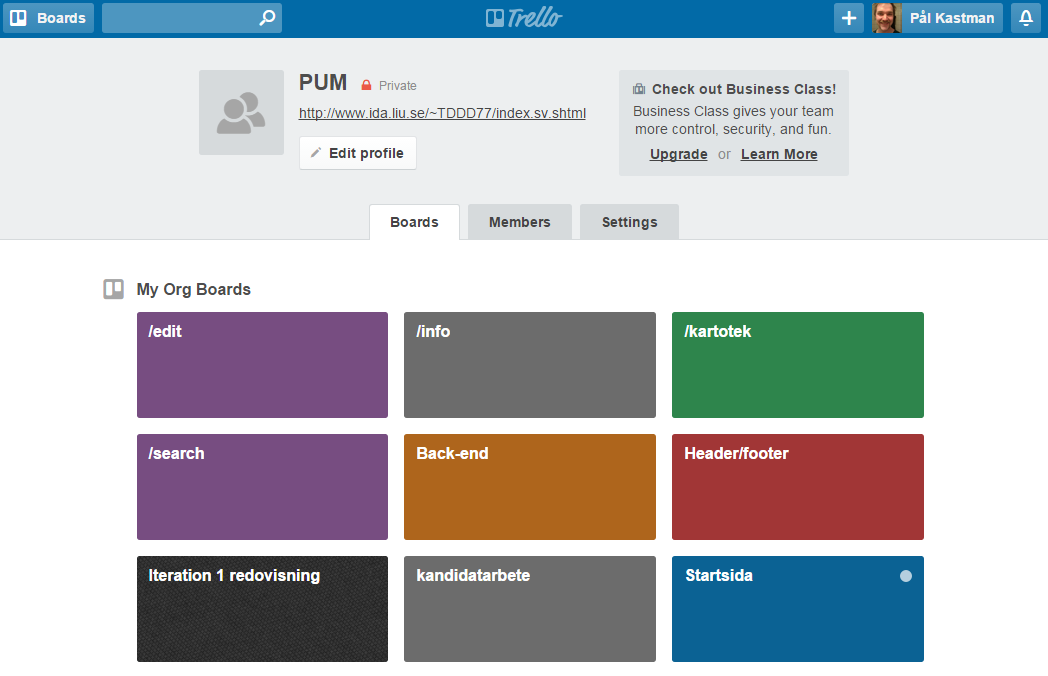
\includegraphics[width=\textwidth]{trello.png}
                \label{fig:gull}
        \end{subfigure}%
        \begin{subfigure}[b]{0.5\textwidth}
                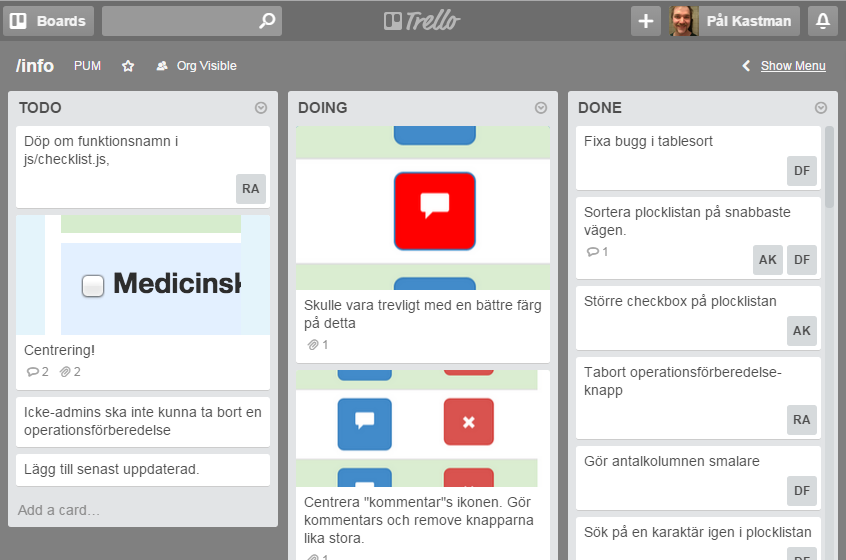
\includegraphics[width=\textwidth]{trello2.png}
                \label{fig:tiger}
        \end{subfigure}
        \caption{Trello, t.v. översikt över alla boards, t.h. boarden info}\label{fig:trello}
\end{figure}

Boarden hade kategorierna TODO, DOING och DONE. När en medlem valt en aktivitet så märktes aktiviteten med medlemmens namn och flyttades till den aktuella kategorin. Varje vecka har gruppen haft ett kort SCRUM-möte på 15 minuter. På mötet har varje gruppmedlem berättat vad som har gjorts den föregående veckan och vad som ska göras nästa vecka. SCRUM-mötet har oftast utförts i samband med varje veckas handledarmöte.

\subsubsection{Alpha state cards}
Ett system med alpha state cards har använts för att gruppen skulle kunna ha koll på hur långt projektet har fortskridit. Korten har även använts till att identifiera aspekter av projektet som kan förbättras och som gruppen behöver arbeta mer med. De aspekter av projektet som kunnat förbättras har använts som mål för kommande iterationer. De olika korten har uppdaterats kontinuerligt under projektets gång.

\subsubsection{Sammarbete i gruppen}
Under förstudien så diskuterades det hur utvecklingen skulle ske på bästa på sätt för gruppen. Förslagen som diskuterades var, utveckling i mindre grupper, separat arbete var för sig eller att alla gruppmedlemmar skulle sitta tillsammans och utveckla. Då alla i gruppen inte hade utvecklat någon webbaplikation tidigare så togs beslutet att under förstudien paralellt inleda en intern utbildning inom gruppen i form av så kallade kodstugor, dessa gick ut på att alla skulle sitta tillsammans och lära sig de olika verktygen så som t.ex. javascript och css och att de mindre erfarna skulle ha en möjlighet att få hjälp av de mer erfarna.


\clearpage
\section{Resultat}
Denna del av dokumentet presenterar resultatet av vårt arbete.
Här kommer beskrivs både hur systemet ser ut och används, samt hur det är uppbyggt rent tekniskt.

\subsection{Översikt av systemet}
Det finns två huvuddelar i systemet. Handböckerna och kartoteket.

Handböckerna beskriver hur man förbereder olika typer av operationer.
Varje handbok har en lista med artiklar som behövs till operationen, en så kallad plocklista.
Artiklarna är kopplade till kartoteket, som bland annat innehåller information om var i förråden artiklarna finns placerade.

När en patient registreras skapas en instans av en handbok.
I denna instans kan man checka av en lista med artiklar som ska användas under operationen och även andra förberedelser.
En samordnare kan se en översikt på hur långt man har kommit med de förberedelserna för varje instans.
Se en översikt i figur \ref{fig:overview}.

\begin{figure}[htbp]
  \centering
  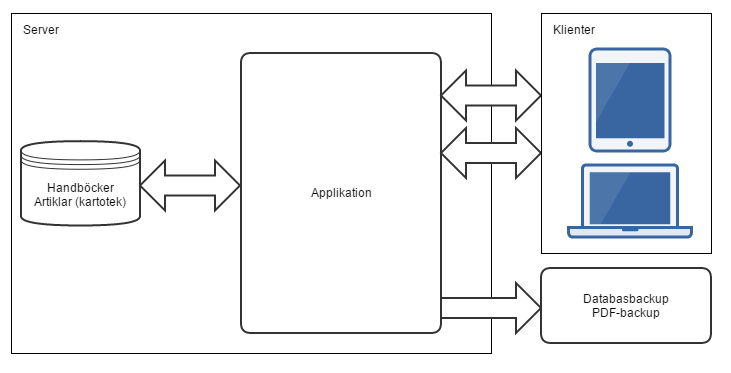
\includegraphics[width=0.9\textwidth]{images/overview.png}
  \caption{Översikt av systemet}
  \label{fig:overview}
\end{figure}

\subsubsection{Server och klient}
Applikationen består av en server som distribuerar en hemsida till flera klienter.
Servern kan köras i en Windowsmiljö.
Hemsidan är responsiv och fungerar på surfplattor och datorer i olika format.

\subsubsection{Kartoteket}
I kartoteket finns information om alla artiklar som Region Östergötland har i förråden.
Här finns bland annat information om var artiklarna är placerade samt information relaterade till inköp av artiklar.

Läs mer om kartoteket i "Kartoteket"\ nedan.

\subsection{Tekniker}
Vi börjar med att beskriva tekniken bakom systemet.

\subsubsection{Översikt}
Programmet är uppdelat i två delar, en serverdel och en klientdel.
Serverdelen består av databaskopplingar som kopplas ihop och distribueras ut genom hemsidor till klienterna.

\begin{figure}
  \centering
  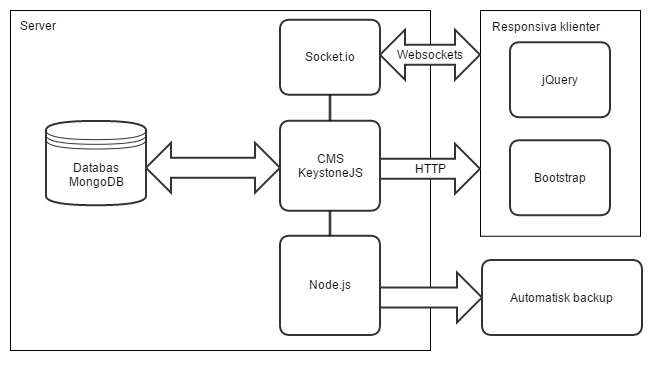
\includegraphics[width=0.9\textwidth]{images/techoverview.png}
  \caption{En översikt över tekniken}
  \label{fig:techoverview}
\end{figure}

I figur \ref{fig:techoverview} kan man se en översikt över de mest betydelsefulla tekniker och bibliotek som används för att bygga upp programmet.

\subsubsection{Back-end}
Koden till servern har skrivits helt i javascript.
Dels för att underlätta inlärningskurvan genom att använda samma språk som på klienten och dels för att realtidskommunikation mellan klienterna underlättas.
Grunden till programmet är node.js vilket är en plattform för att utveckla självständiga program i javascript med inbyggd pakethanterare.
Pakethanteraren gör det enkelt att installera externa bibliotek.

Det största och mest betydelsefulla ramverket för detta projekt är KeystoneJS, ett CMS-ramverk till node.js.
Följande är några punkter KeystoneJS underlättar:
\begin{itemize}
  \item Hjälper till att abstrahera systemet. Se avsnittet om MVC nedan.
  \item Skapar automatiskt en administreringssida för varje databasmodell.
    Huvuddelen av administeringen har dock bytts ut då den automatgenererade kan vara något begränsad.
  \item Har ett inbyggt användarsystem som är lätt att modifiera och byta ut.
  \item Sköter all kommunikation över http-protokollet till klienterna, dvs. gör hemsidan åtkomlig.
  \item Har inbyggt stöd för templatespråk som exempelvis Handlebars\footnote{TODO: bättre referens. http://handlebarsjs.com/ (2015-04-18)} och Less\footnote{TODO: Bättre referens. http://lesscss.org/ (2015-04-18)}.
\end{itemize}

För realtidskommunikation används ett programmeringsinterface vid namn socket.io\footnote{TODO: bättre referens. http://socket.io/ (2015-04-18)} användas.
Det är väldigt smidigt eftersom det väljer automatiskt hur datan ska skickas beroende på vilken webbläsare som används och vad den stödjer.
Socket.io är event-baserat vilket betyder att man skapar events på antingen klient eller serversida som man sedan kan trigga från motsatt sida.
Vanliga javascript-object kan skickas tillsammans med eventen.

\subsubsection{Front-end}
På klientsidan används bootstrap\footnote{TODO: Bättre referens.} och jQuery\footnote{TODO: Bättre referens.}.
Bootstrap har många färdiga CSS-klasser så man behöver inte skriva lika mycket CSS själv.
De klasser som finns är lätta att använda för att skapa responsiva hemsidor.
All kod är dessutom testad för att fungera på olika webbläsare vilket kan vara krångligt att lösa om man skriver all CSS från grunden.
JQuery används för att lättare hämta ut ett element på hemsidan och ändra data i det.
Det finns även många bra jQuery-bibliotek att hämta som gör att man slipper “uppfinna hjulet” i många fall.

För att ytterligare design av hemsidan används LESS\footnote{TODO: Referens.} att användas.
Det är en påbyggnad till CSS som kompilerar till vanliga CSS-filer.
Fördelen med LESS är bland annat att man kan använda variabler och enkla funktioner.
Exempelvis kan variablerna användas för att spara de olika färgerna på hemsidan för att enkelt kunna byta ut dem.


\subsubsection{Struktur}
En nackdel med jQuery gentemot andra bibliotek som exempelvis angular\footnote{TODO: Referens.} är att det lätt blir spaghettikod\footnote{TODO: Måste defineras?}.
För att strukturera så bra som möjligt är det viktigt att koden uppdelad.
För att uppnå detta så kommer varje enskild sida ha minst en skriptfil, en cssfil och en htmlfil.
På vissa sidor är det lätt att det blir stora skript och då bör man dela upp skriptfilen.
Den bästa lösningen är att abstrahera delar av skriptet till egna biblioteksfiler som man kan ladda in och använda.

\subsubsection{Säkerhetskopiering och reservsystem}
Det ställs stora krav på att handböckerna alltid ska finnas tillgängliga då de ska användas på ett sjukhus där ett fel kan få stora konsekvenser. Detta innebär att ett reservsystem måste finnas till hands ifall systemet slutar fungera. Detta har lösts genom ett system där pdf-kopior av handböcker skapas. Handböckerna hamnar i en mapp-struktur där de sorteras på specialitet och operation. Kopian sparas med ett versionnummer, vilket gör att kopior av gamla versioner av operationer fortfarande finns kvar och kan skrivas ut. Var denna mapp-strukturen ska hamna bestäms i en konfigurationsfil.
Kopiorna skapas genom att en funktion, som kollar igenom alla handböcker för att se om har uppdaterats sedan senaste kopieringen, körs med ett givet tidsintervall som ställs in i konfigurationsfilen. Om en operation har uppdaterats så körs en funktion som använder en modul, som heter wkhtmltopdf, för att kalla på ett program som också heter wkhtmltopdf. Wkhtmltopdf använder en osynlig webbläsare för att skapa en pdf-kopia. Hur kopiorna ser ut kan ses i figur \ref{fig:pdf-start} och figur \ref{fig:pdf-end}. Utseendet ändras genom att speciell css för utskrift finns och wkhtmltopdf körs med utskrift som mediatyp. 
Det finns också ett REST-api för att skapa pdf-kopior. Detta används dock inte någonstans. Men en vidareutveckling på detta vore att implementera att en ny pdf-kopia skapas så fort en operation har uppdaterats. 

\begin{figure}
  \centering
  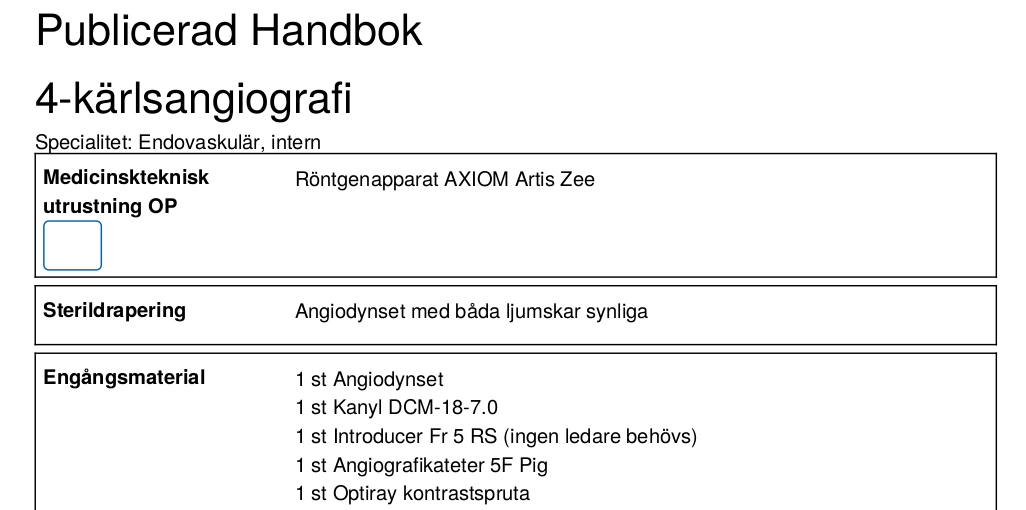
\includegraphics[width=0.9\textwidth]{images/pdf-start.png}
  \caption{Början på en pdf-kopia.}
  \label{fig:pdf-start}
\end{figure}

\begin{figure}
  \centering
  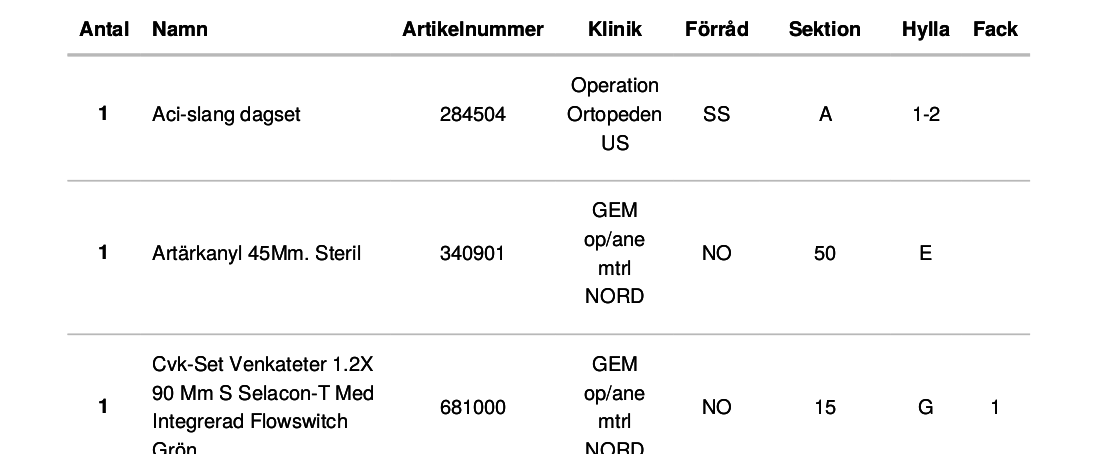
\includegraphics[width=0.9\textwidth]{images/pdf-end.png}
  \caption{Plocklista i en pdf-kopia.}
  \label{fig:pdf-end}
\end{figure}

Det krävs mycket arbete för att lägga in alla handböcker, vilket gör att det är viktigt att databasen säkerhetskopieras med jämna mellanrum. Med ett givet tidsintervall som går att ställa in i konfigurationsfilen så körs en funktion som använde en modul som heter mongo-utils för att kalla på mongodump som tar en kopia på databasen och lägger den i en mapp med dagens datum. 
\subsection{Mekanismer}
Här beskrivs syftet och funktionalitet hos olika delar av produkten.

\subsubsection{Översikt}
Som tidigare nämnts finns en översikt över alla operationsförberedelser.
Denna sida visar alla operationsförberedelser och hur långt är fortskridna.
Här används Socket.IO för att hela tiden hålla information uppdaterad.

\begin{figure}[h!]
  \centering
  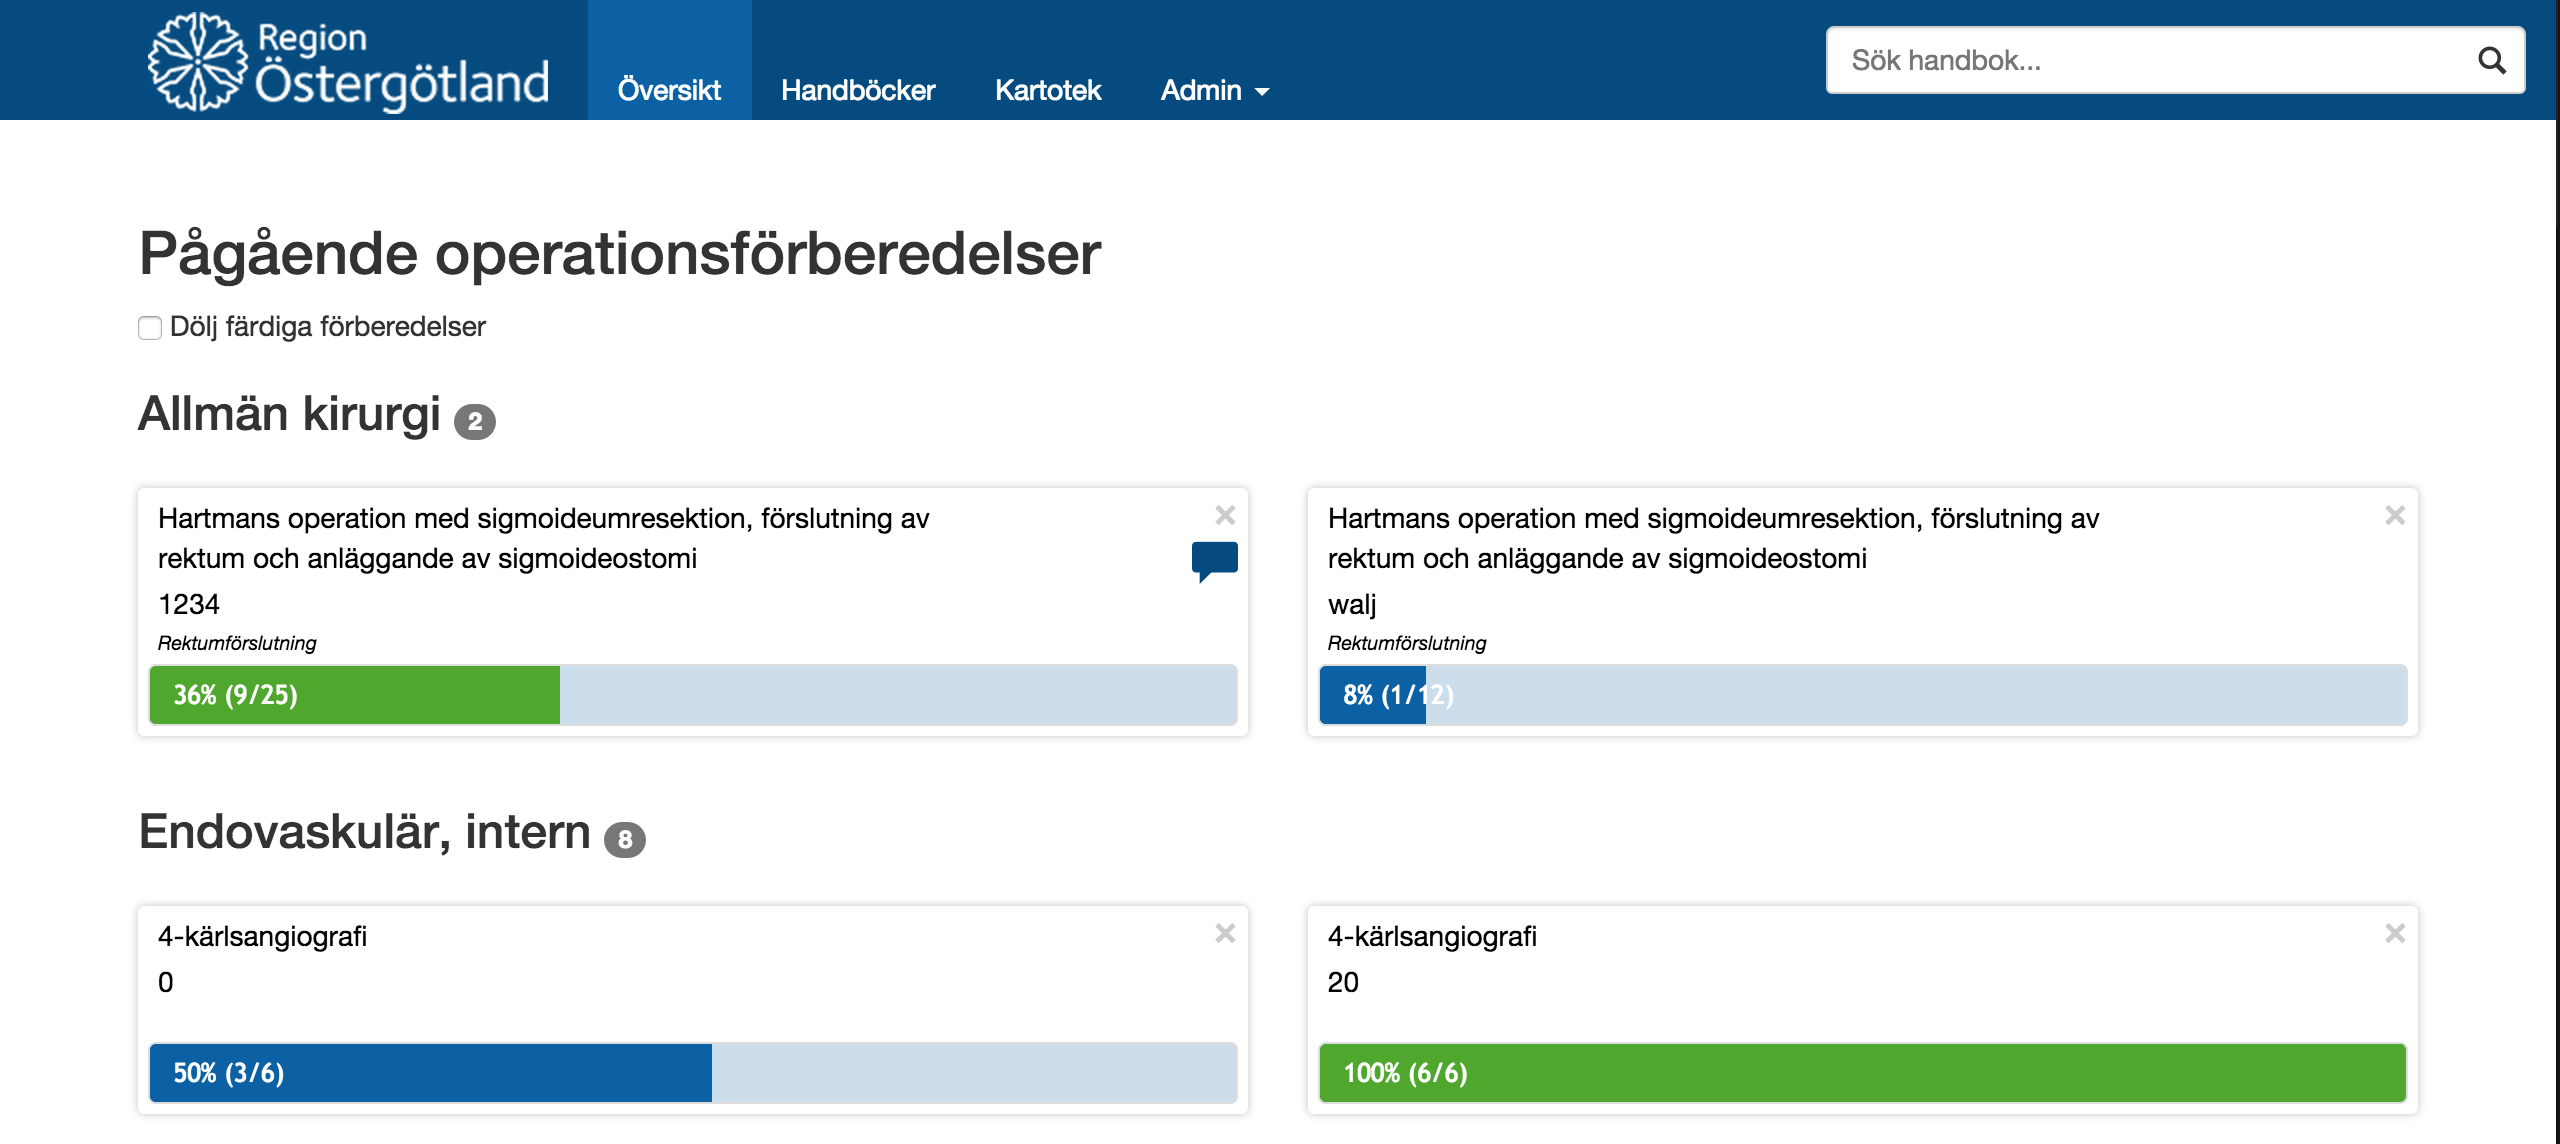
\includegraphics[width=0.95\textwidth]{images/site/overview.png}
  \caption{Bild på översiktsvyn}
  \label{fig:siteoverview}
\end{figure}

I figur \ref{fig:siteoverview} kan man se hur förberedelserna är kategoriserade beroende på vilken kirurgisk specialitet handboken tillhör.
Ibland är det olika samordnare beronde på specialitet och det är då enkelt för en samordnare att hitta de operationerna som personen är ansvarig över.

\subsubsection{Handbok}
En handbok innehåller information om en operationsförberedelse.

\begin{figure}
  \centering
  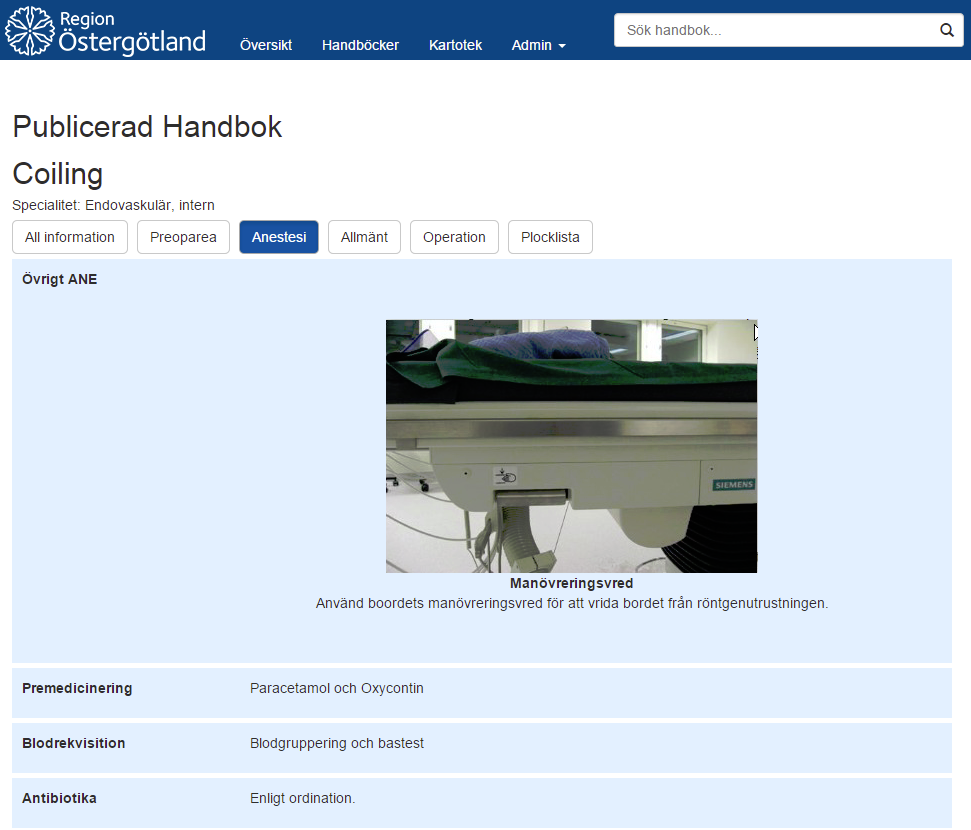
\includegraphics[width=0.9\textwidth]{images/site/handbok.png}
  \caption{En handbok}
  \label{fig:handbok}
\end{figure}

All information i en handbok är uppdelad i olika rubriker. Dessa rubriker kan i sin tur vara uppdelade i olika processer.
I figur \ref{fig:handbok} ser man dels de olika processerna (Preoparea, anestesi, allmänt och operation) samt rubrikerna som hör till processen Anestesi (Övrigt, Premedicinering, blodrekvisition och  antibiotika).
Man kan även se att handböckerna har stöd för bilder.

\subsubsection{Sökfunktion}
Ett krav är att det ska vara lätt att hitta en handbok.
Därför kan man söka både på operationens namn men även på alternativa sökord (taggar), dessa är bra att ha då de medicinska termerna ibland kan vara svåra att komma ihåg.

\begin{figure}
  \centering
  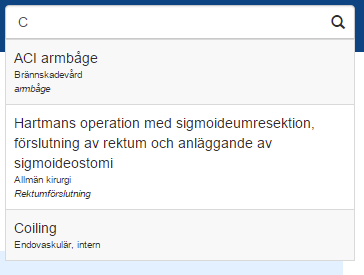
\includegraphics[width=0.9\textwidth]{images/site/search}
  \caption{Sökfunktionen}
  \label{fig:search}
\end{figure}

I figur \ref{fig:search} kan man se sökresultaten där namnet på operationen står i större storlek, och sökorden kursivt i mindre storlek.

\subsubsection{Lista med handböcker}
Applikationen innehåller en enkel lista med alla handböcker.
Den går att sortera på valfri kolumn och kan även gruppera beroende på vilken specialitet handboken tillhör.
Se figur \ref{fig:list}

\begin{figure}
  \centering
  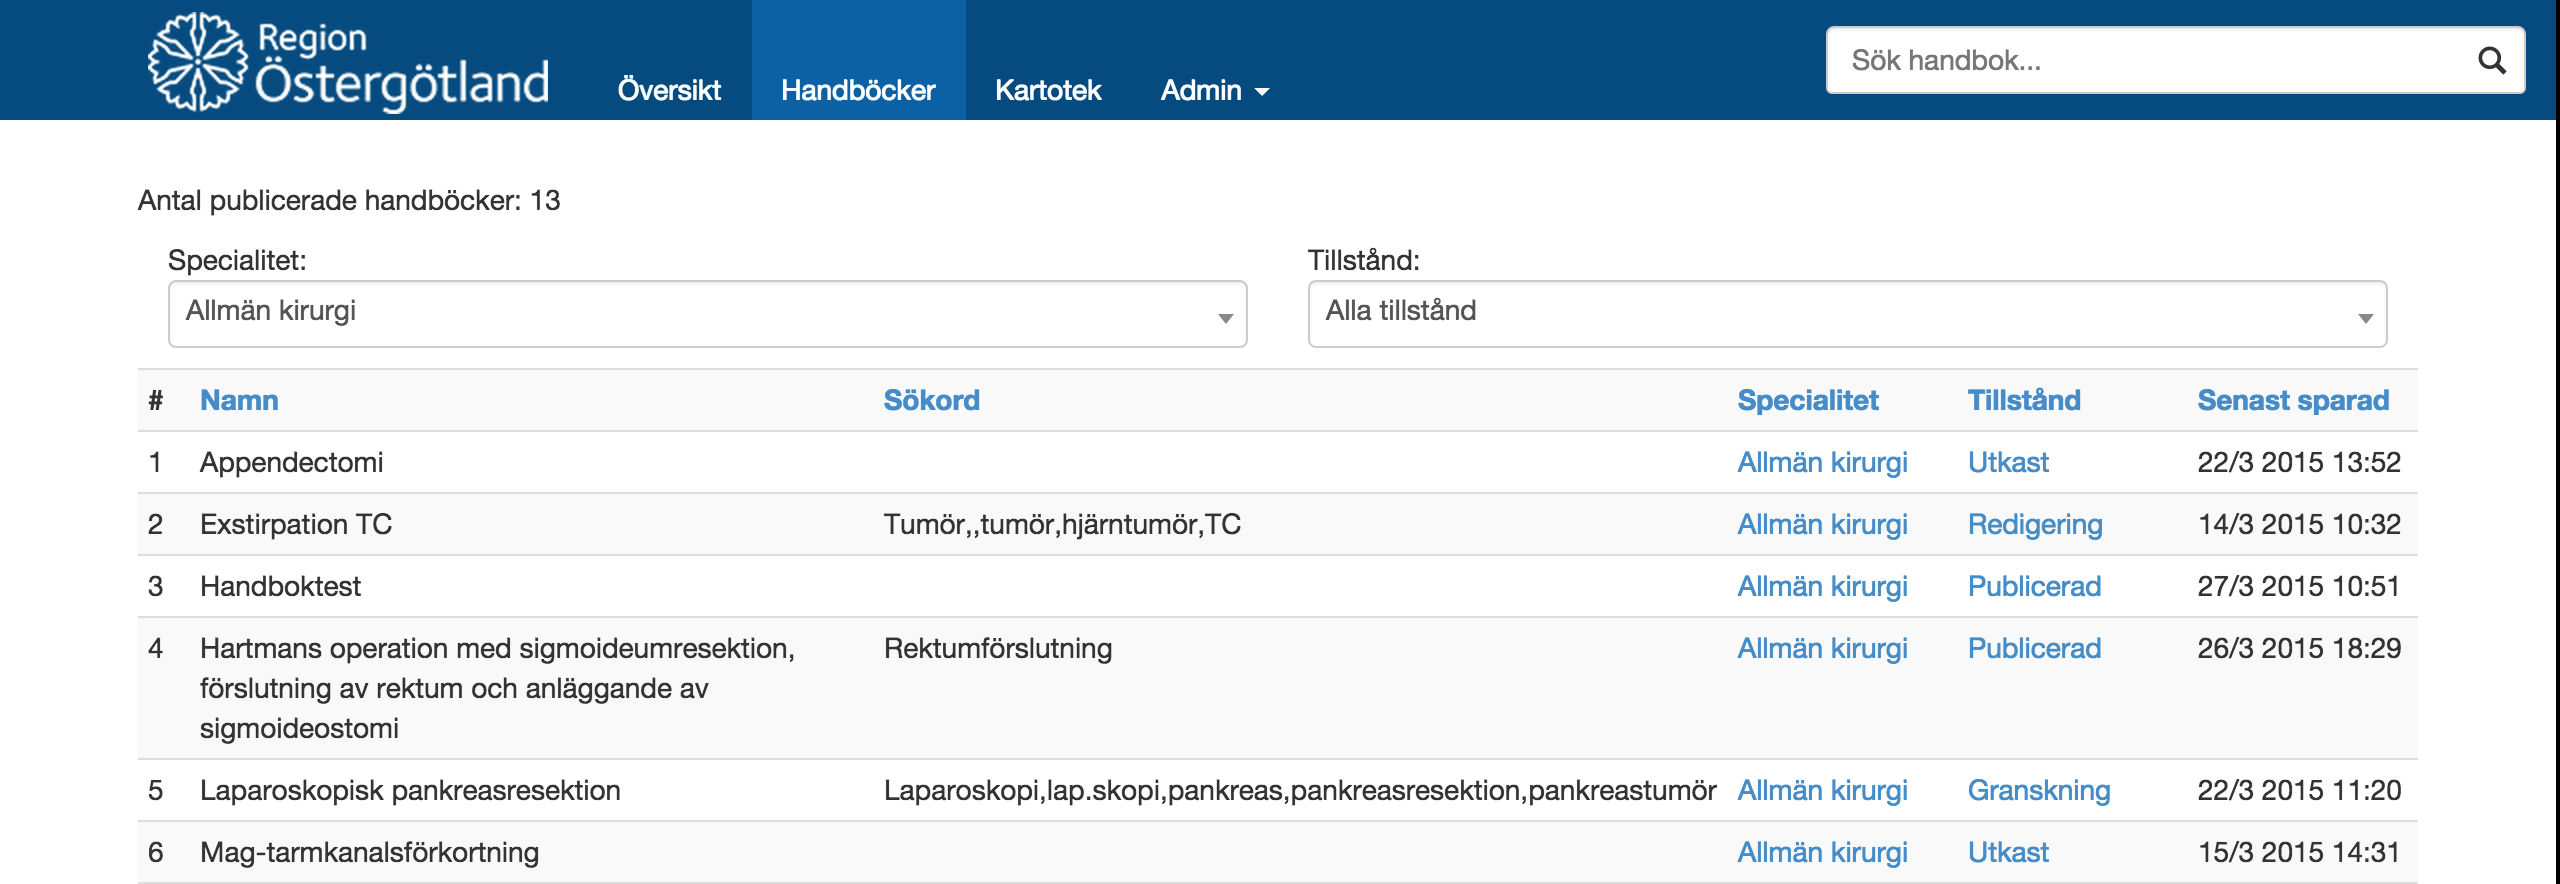
\includegraphics[width=0.95\textwidth]{images/site/list}
  \caption{Lista med handböcker}
  \label{fig:list}
\end{figure}

\subsubsection{Administrering}
I administreringsvyn kan man utöver att redigera all information även sortera processer och rubriker genom att dra och släppa dem.
Redigeringen under rubrikerna använder sig av en wysiwyg-editor.
Innan en redigerad eller ny handbok publiceras måste den granskas av en annan person.

\subsubsection{Operationsförberedelse}
En operationsförberedelse är nästan likadan som en handbok.
Det som skiljer är att vissa av rubrikerna kan gå att kryssa av när de är klara.

\begin{figure}
  \centering
  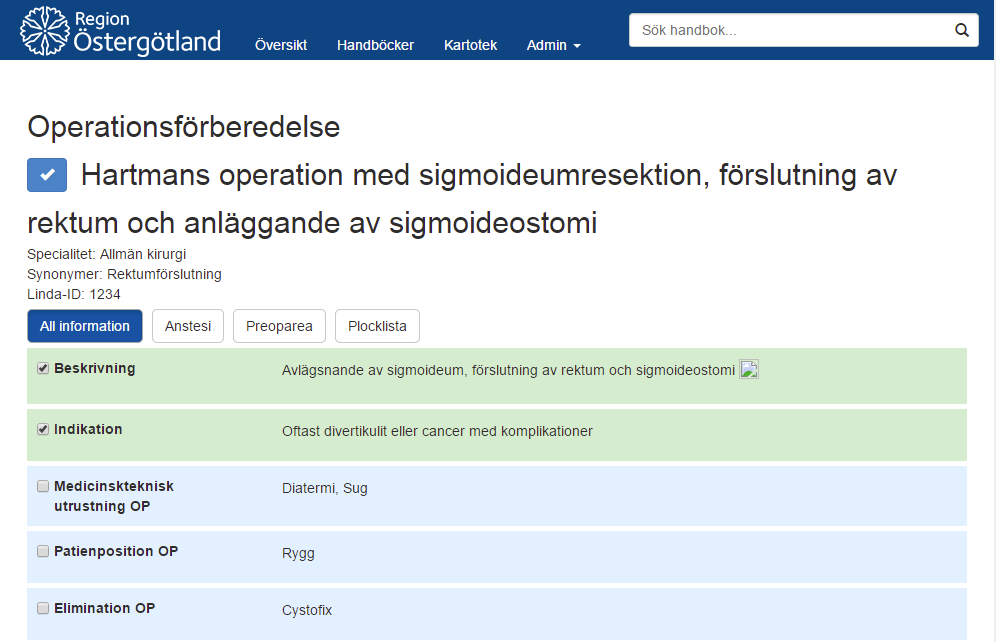
\includegraphics[width=0.9\textwidth]{images/site/op}
  \caption{Förberedelsevyn}
  \label{fig:op}
\end{figure}

I figur \ref{fig:op} kan man se att rubrikerna går att kryssa av när de är klara. Jämför med figur \ref{fig:handbok} där rubrikerna inte går att kryssa av.

\subsubsection{Plocklista}
En operationsförberedelse har även en plocklista med artiklar som behövs till operationen.

\begin{figure}
  \centering
  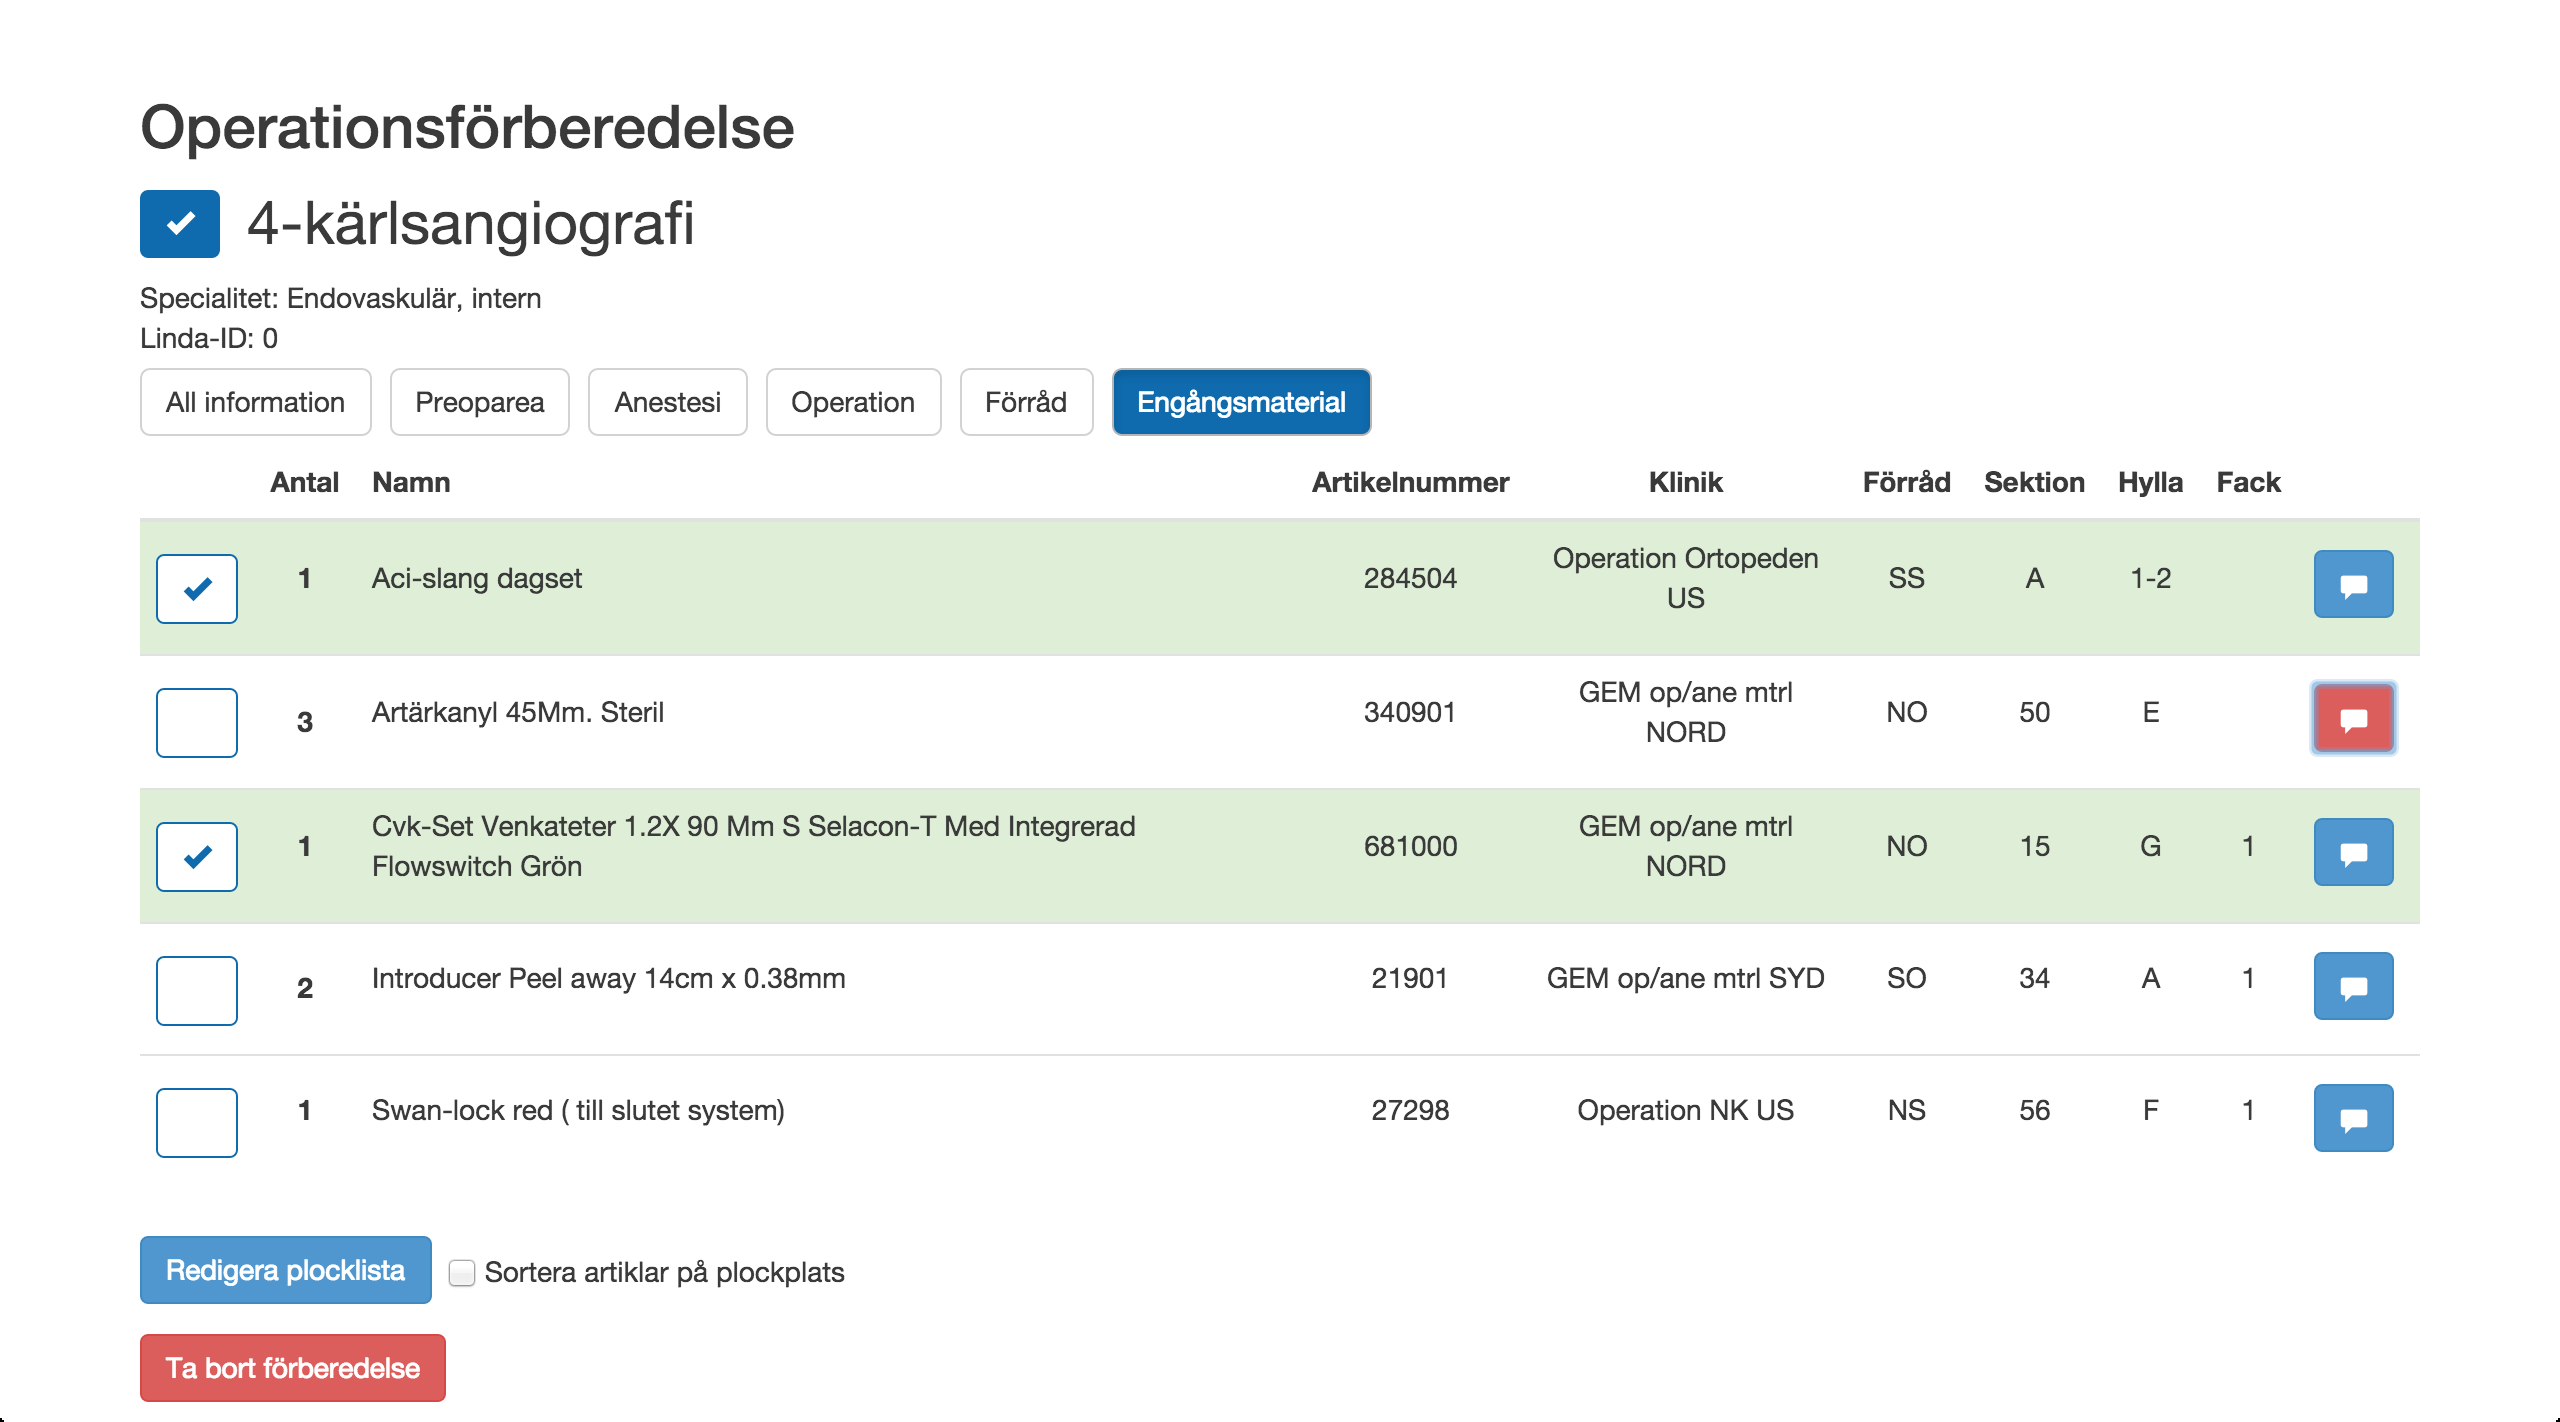
\includegraphics[width=0.9\textwidth]{images/site/plocklista}
  \caption{Plocklista}
  \label{fig:plocklista}
\end{figure}

I figur \ref{fig:plocklista} kan man även se att det finns stöd för att lägga en kommentar på en artikel.
Det är vanligt att en artikel är slut eller utbytt och man kan då lägga en kommentar på varför man inte kunde hämta den artikeln och även hur man har löst det istället.

\subsubsection{Kartoteket}
Kartoteket diskuteras i djup detalj nedan.

\subsubsection{Publicering och granskning}
Flöded för att skapa en handbok involverar flera steg.
Se figur för en övervy.

\begin{figure}
  \centering
  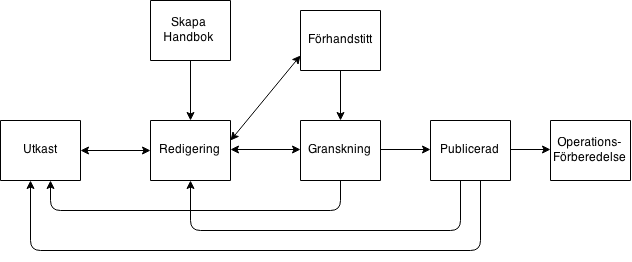
\includegraphics[width=0.7\textwidth]{images/model}
  \caption{Publicering och granskining}
  \label{fig:model}
\end{figure}

När man först vill skapa en handbok så hamnar man i ett redigeringsläge,
där man kan lägga till information om handboken, som artiklar i plocklista,
beskrivning av operationen.
Härifrån kan man välja att förhandsgranska, för att se om den ser ok ut,
eller skicka till granskning, där den går vidare till publicering
efter någon annan läst igenom materialet och de tycker det ser rätt ut.
Om man har en handbok i redigeringsläge som inte är klar så hamnar den även i
"utkast"-läge, likt en email-system.
Slutligen kan en publicerad handbok gå vidare till att bli en
operationsförberedelse om det är dags att utföra en sådan operation
som beskrivs i handboken.

\subsection{Utvecklingen}
Här nedan beskrivs resultatet av hur utvecklingen inom gruppen har fungerat,
och huruvida de olika hjälpmedlen har hjälpt eller stjälpt.

\subsubsection{SCRUM}
Utvecklingen i SCRUM-form har fungerat bra,
dock har utvecklingen som beskriven i metod inte varit i rent SCRUM-format utan har modifierats för att bättre passa gruppen.
Ett möte med handledare har hållits en gång i veckan där handledaren har haft möjlighet att ta upp saker som denne tyckt har behövts,
sedan har gruppen hållit ett kort SCRUM-möte där man fått förklara vad man gjort förra veckan och vad man planerat
att göra kommande vecka. Under mötets gång har man noterat om det är någonting som har behövt diskuteras
vidare och detta har då noterats, varpå gruppen har gått igenom dessa frågor efteråt. Detta har fungerat väldigt bra då man på detta sättet inte har fått några större avbrott och alla hela tiden kunna hålla fokus. Efter SCRUM-mötena så har ordet varit fritt och alla har haft möjligheten att komma med synpunkter eller åsikter över någonting.

\subsubsection{Alpha state cards}
Korten har kontinuerligt uppdaterats av teamledare, dock har de kanske inte använts lika flitigt av gruppen som tanken var att de skulle?

\subsubsection{Kundmöten}
I inledningen hölls totalt fyra möten, det första var ett längre möte, där endast teamledaren, kundansvarige och arkitekten närvarade från projektgruppen. Detta möte hölls främst som en introduktion men var även ett tillfälle för kunden att visa upp sitt nuvarande system och få framföra ideér om hur system skulle kunna se ut och fungera istället. Sedan gjordes ett studiebesök hos kunden där alla gruppmedlemmar deltog. Man fick se hur en sjuksköterska förberedde inför en operation och även se deras nuvarande system i bruk. Under det tredje mötet så utformade man kravspecifikationen som man sedan spikade under det fjärde mötet.

Efter varje iteration hölls ett möte på plats hos kunden för att diskutera hur arbetet fortskred, detta var även ett perfekt tillfälle att ta upp saker man var osäker kring, men var även bra för båda parter att föreslå ändringar i systemet. Mötet efter iteration två bestämdes att det skulle sättas upp en server där kunden skulle kunna testköra systemet, det bestämdes också att några från projektgruppen skulle närvara vid dessa tester. Detta gjordes två gånger där arkitekt och kundansvarige medverkade vid första tillfället, kvalitetsansvarige och dokumentansvarige medverkade vid det sista tillfället

\subsubsection{Samarbete i gruppen}
Samarbetet i gruppen har fungerat väldigt bra, kodstugorna som gruppen höll under förstudien var alla nöjda med, de som var mindre erfarna med webbprogrammering kände att de fick all den hjälp de behövde när de körde fast i sitt arbete och därför kändes det naturligt för hela gruppen att fortsätta med dessa även under utvecklingsfasen.

%\subsection{Gruppens gemensamma erfarenheter}
%\subsection{Översikt över de inviduella utredningarna}

\clearpage

\section{Diskussion}

\subsection{Resultat}

\subsection{Metod}
Metoden som användes för kravframställning fokuserade på att i förstudien samla in så mycket krav som möjligt genom möten, intervjuer och obeservationer. Att arbeta fram kraven tillsammans med kund kändes nödvändigt för att få en fullständig bild. En sak som vi inte prioriterades men som kanske hade kunnat hjälpt arbetet skulle varit att lägga större fokus på olika roller. Slutsystemet har två roller vilket är admins och icke-admins. En avvägning gjordes där dessa två enkla roller valdes. Fördelen var att att vi kunde lägga fokus på att snabbare kunna testa andra delar av systemet med högre prioritet. Nackdelen var att dessa funktionaliteter inte hann testas och under förstudien ledde till en viss förivirring. %%blablabla
Att använda use-cases eller user-stoires diskuterades också under förstudien. Detta bortprioriterades då vi ansåg att de var överflödiga. Denna avvägning ledde till att det var lite svårare att kommunicera kraven. 

\subsection{Arbetet i ett vidare sammanhang}

\section{Slutsatser}

\section{Fortsatt arbete}
Här följer en sammanfattning om fortsatt arbete med systemet. Restlistan behandlar krav som inte implementerats eller som borde vidareutvecklas. Även förslag på vidareutveckling som inte tas upp av kravspecifikationen tas upp. Dessa förslag är sådant som kommit fram under utvecklingens gång.

\subsection{Restlista}
Följande krav är markerade som gula i kravspecifikationen vilket betyder att de bör vidareutvecklas för att ses som klara:
%%Fyll på gula krav här efter iteration 3 mötet
Följande krav är markerade som röda i kravspecifikationen vilket betyder att de inte är påbörjade:
%%Fyll på röda krav här efter iteration 3 mötet
Alla krav som behandlar lagersystemet finns kvar:
\begin{description}
\item[Krav nr 46] Ska finnas ett saldo för varje artikel i förrådet.
\item[Krav nr 47] Ska gå att skanna av artiklar (streckkod) som plockas i en specifik plocklista.
\item[Krav nr 48] Ska gå att lagra in en artikel till förrådet som inte blivit använd genom att skanna in den.
\item[Krav nr 49] Saldot ska kunna användas som underlag till beställning.
\item[Krav nr 50] Beställningsunderlaget ska ha ett sådant format att det går att importera i Agresso.
\item[Krav nr 51] En inventeringsfunktion ska finnas.
\end{description}

Övriga förslag på vidareutveckling:
%%Fyll på här om ni kommer på något!


\begin{description}
\item[Artikelsök] Vid sökning på artikel vid redigering av handbok kan det vara bra om man sorterar resultaten så att de artiklar som tillhör samma enhet som handboken visas först.
\item[Avancerad sökfunktion] En mer avancerad sökfunktion med * och söknining på flera ord som inte behöver vara direkt efter varandra.
\item[Förvalda kommentarer] Under användartester observerades att samma kommentarer skrivs ofta så det kan vara bra med en lista på vanliga kommentarer som man kan välja ifrån.
\item[Roller och rättigheter] Olika roller bör identifieras och en funktion för att tilldela användare olika rättigheter bör implementeras.
\end{description}
\subsection{Referenser}
\begin{thebibliography}{9}
\bibitem{Elisabeth}
Får nog fixa en bättre referens här.
\end{thebibliography}

\newpage
\part{Enskilda utredningar}
\renewcommand{\thesection}{\Alph{section}}	
\section{Kartoteket - Daniel Rapp}
\subsection{Inledning}
Idag är information om Region Östergötlands operationsartiklar, så som priserna och
placeringen i lagret på tandborstar, tandkräm, handskar och annan
medicinsk utrustning, hanterat av ett internt system.
Detta system kallas ett "\textit{kartotek}", och är helt enkelt en sorts artikeldatabas.
I vårt system så ska detta uppdateras och förbättras på olika sätt.

\subsubsection{Syfte}
Syftet med denna del är att beskriva vad kartoteket är samt
hur vår förbättrade lösning är uppbyggd.


\subsubsection{Frågeställning}
Frågeställningar:
\begin{itemize}
  %\item Kan man implementera ett kartotekssystem som uppfyller kundens önskemål?
  %\item Går det att implementera ett kartotekssystem som 
  \item Går det att integrera systemet för handböcker med kartoteket utan att förlora funktionalitet?
\end{itemize}


\subsubsection{Avgränsningar}
Förutom ett förbättrat kartotekssystem så är Region Östergötland också i behov av
ett bättre system för att hantera deras lager på ett mer automatiserat sätt.
Bland annat så skulle de behöva ett system som låter dem checka in vilka varor från lagret de hämtat
ut, istället för att checka av manuellt, vilket kan vara felbenäget.

Vi valde dock att avgränsa oss från att bygga denna lösning, på grund av tidsbrist.
Istället fokuserade vi på att förbättra kärnfunktionaliteten i applikationen.


\clearpage
\subsection{Bakgrund}
I dagsläget använder Region Östergötland sig av två separata system
för att förbereda operationer. En handbok (se ovan) och ett kartotek (se figur \ref{fig:kartotek}).
Dessa är för tillfället helt separata applikationer.

\begin{figure}[h!]
  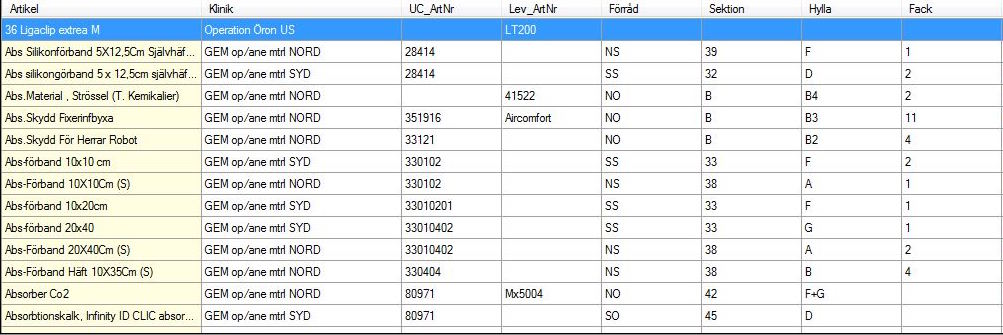
\includegraphics[width=0.9\textwidth]{../images/forradsinfo.jpg}
  \caption{Gamla kartoteket}
  \label{fig:kartotek}
\end{figure}

Så om en artikel har utgått eller Region Östergötland
väljer att inte köpa in en viss artikel längre så tar de bort artikeln
från kartoteket. Problemet som då uppstår är att detta inte reflekteras
i handböckerna. Så om t.ex. en "\textit{Oral-B Pro 600 CrossAction}"\ tandborste används i
en "\textit{Laparoskopisk sigmoideumresektion}", och tandborsten utgår
så tas den bort från kartoteket, men eftersom handboken för operationen inte är
kopplad till kartoteket så uppdateras det inte att denna artikel inte längre finns i lagret.

Vår förbättrade lösning
integrerar systemet som hanterar handböcker tillsammans med ett nytt kartotek,
där allt är byggt på webben. När en artikel ändras eller tas bort i kartoteket
så ändras den även i alla handböcker för operationer som kräver denna artikel.



%\subsection{Teori}
\subsection{Metod}
Precis som resten av systemet så är kartoteket skrivet på webben, och
därmed i javascript, HTML och CSS.
Vi har även använt Git för versionshantering.

Jag måste också nämna att trots att det är jag som skriver om kartoteket,
så är det inte endast jag som har implementerat det. Koden och gränssnittet har givetvis
varit ett stort grupparbete mellan alla medlemmar.


\clearpage
\subsection{Resultat}
Resultatet av vårt arbete är ett förbättrat kartotekssystem
som integrerar data från handboken till ett uniformt system.

Kärnfunktionaliteten i kartoteket är möjligheten att se, modifiera och hitta artiklar.
Så resultatet kommer presenteras i tre delar.

\subsubsection{Att se artiklarna}
När man först kommer in på sidan för att hantera kartoteket så
blir man välkomnad av en stor tabell som innehåller alla artiklar
i kartoteket (runt 3000 för tillfället). Se figur \ref{fig:table}.

\begin{figure}[h!]
  \centering
  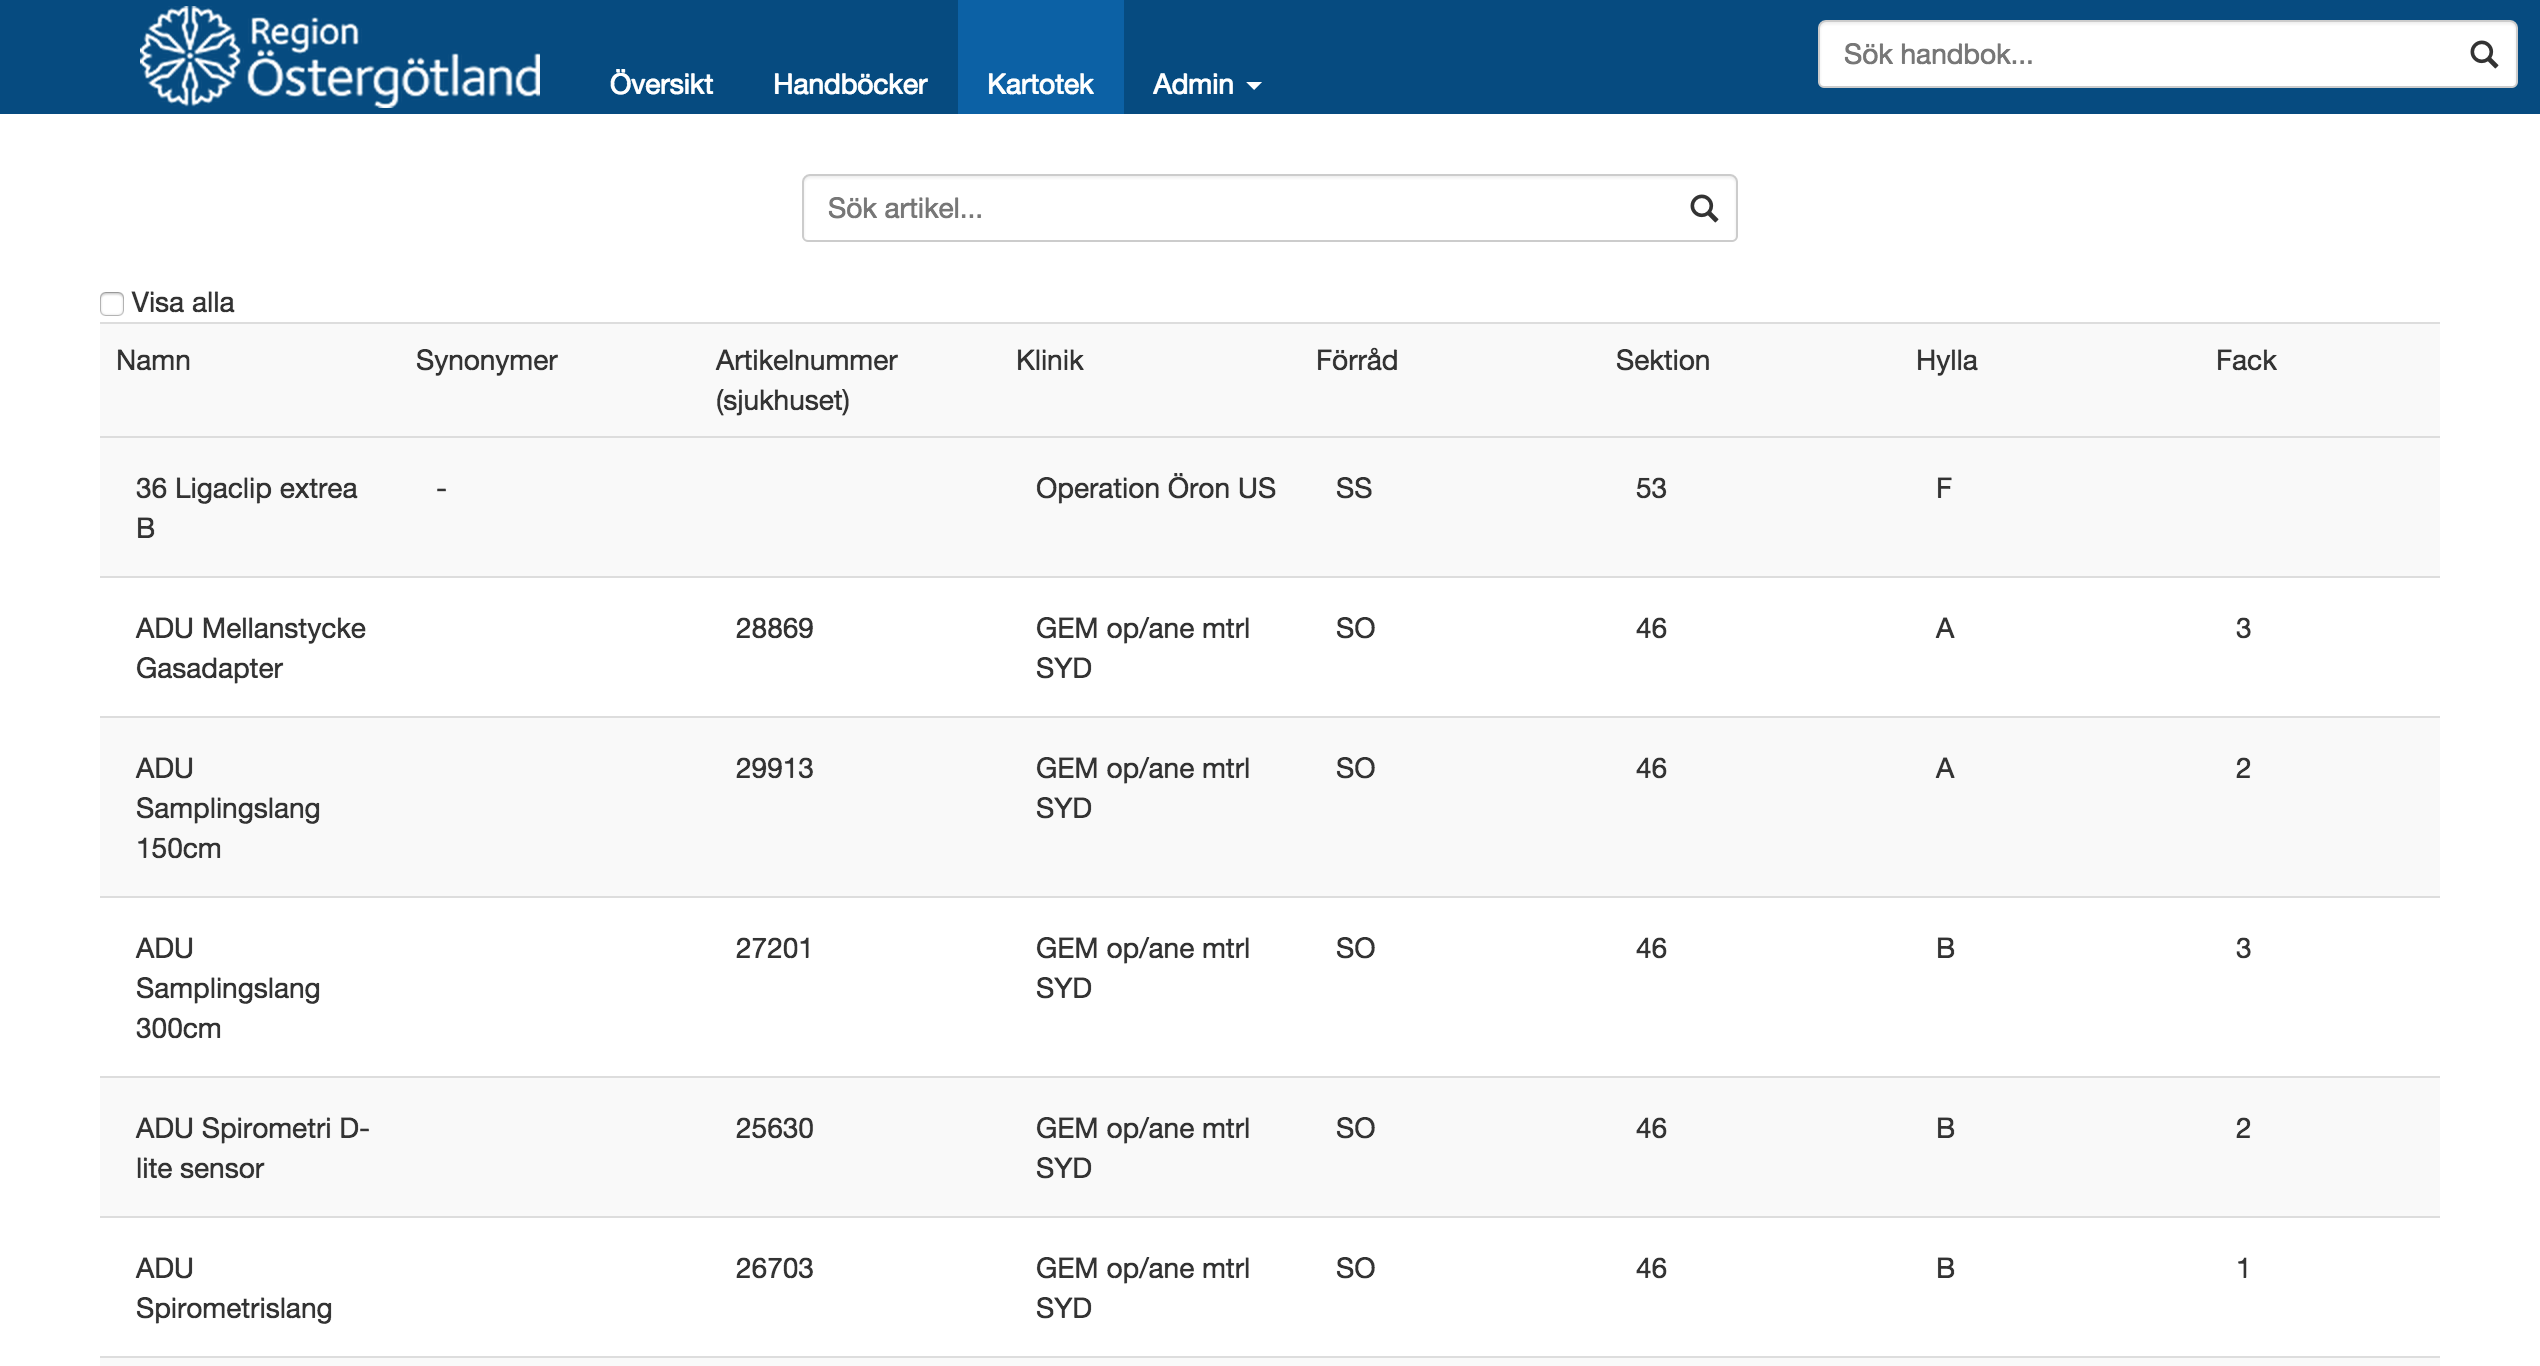
\includegraphics[width=0.9\textwidth]{../images/kartotek1.png}
  \caption{Kartoteket}
  \label{fig:table}
\end{figure}

Först laddas endast runt 50 artiklar, men
om man skrollar ner så laddas fler.

Det finns två olika sätt att se informationen.
Två olika vyer.

Den ena är standardvyen, som man ser om man inte är inloggad
eller inte är administratör. Denna vyn kan ses i figur \ref{fig:table}
och innehåller endast den mest nödvändiga informationen om
artiklarna, som namn, klinik, förråd, etc.

Den andra vyn är administratörsvyn.
Man kommer endast in på denna vy om man är administratör.
Om man aktiverar denna så utvidgas tabellen för att
visa mer information om artiklarna, bland annat pris på artiklarna.
Vi har valt att inte inkludera en bild på denna information
då detta är sekretessbelagt.

I den här vyn finns också möjligheten att ta bort, lägga till och modifiera
information om artiklar, vilket är vad de två följande delarna handlar om.

\clearpage
\subsubsection{Modifiering av artiklarna}
För att modifiera artiklar så måste man som sagt vara administratör.

Med vårt gränssnitt så är det enkelt att modifiera information om en artikel.
Om man vill ändra på, t.ex., artikelnamnet så är det bara att klicka på det!
En input-ruta kommer då upp som låter dig ändra namnet till någonting mer passande.
Detta är inspirerat av Trello, som vi använder för att organisera saker att göra.
I Trello så finns en liknande funktionalitet för att ändra namn på olika "\textit{Boards}".

För att ta bort artiklar så finns det ett smidig "X" till vänster om artikel-raden.

Vi har valt att göra en del av den här informationen obligatorisk, eftersom
sjukhuset hade problem i sitt tidigare system att vissa sjuksköterskor skippade
att skriva in en del viktig information om artikeln.


\subsubsection{Sökning av artiklarna}
Sista kärnfunktionaliteten i kartoteket är sökning.
Eftersom artiklarna är sorterade i bokstavsordning,
och kartoteket har en "infinite scroll"-funktionalitet,
så går det i teorin att hitta alla artiklar utan att söka.
I våra diskussioner kunden på sjukhuset så
verkar det också som det finns vissa personer som primärt använder
sig av denna metod för att hitta artiklar.
Däremot är detta inte en speciellt effektiv lösning, så därför
har vi valt att implementera en sökfunktion.

\begin{figure}[h!]
  \centering
  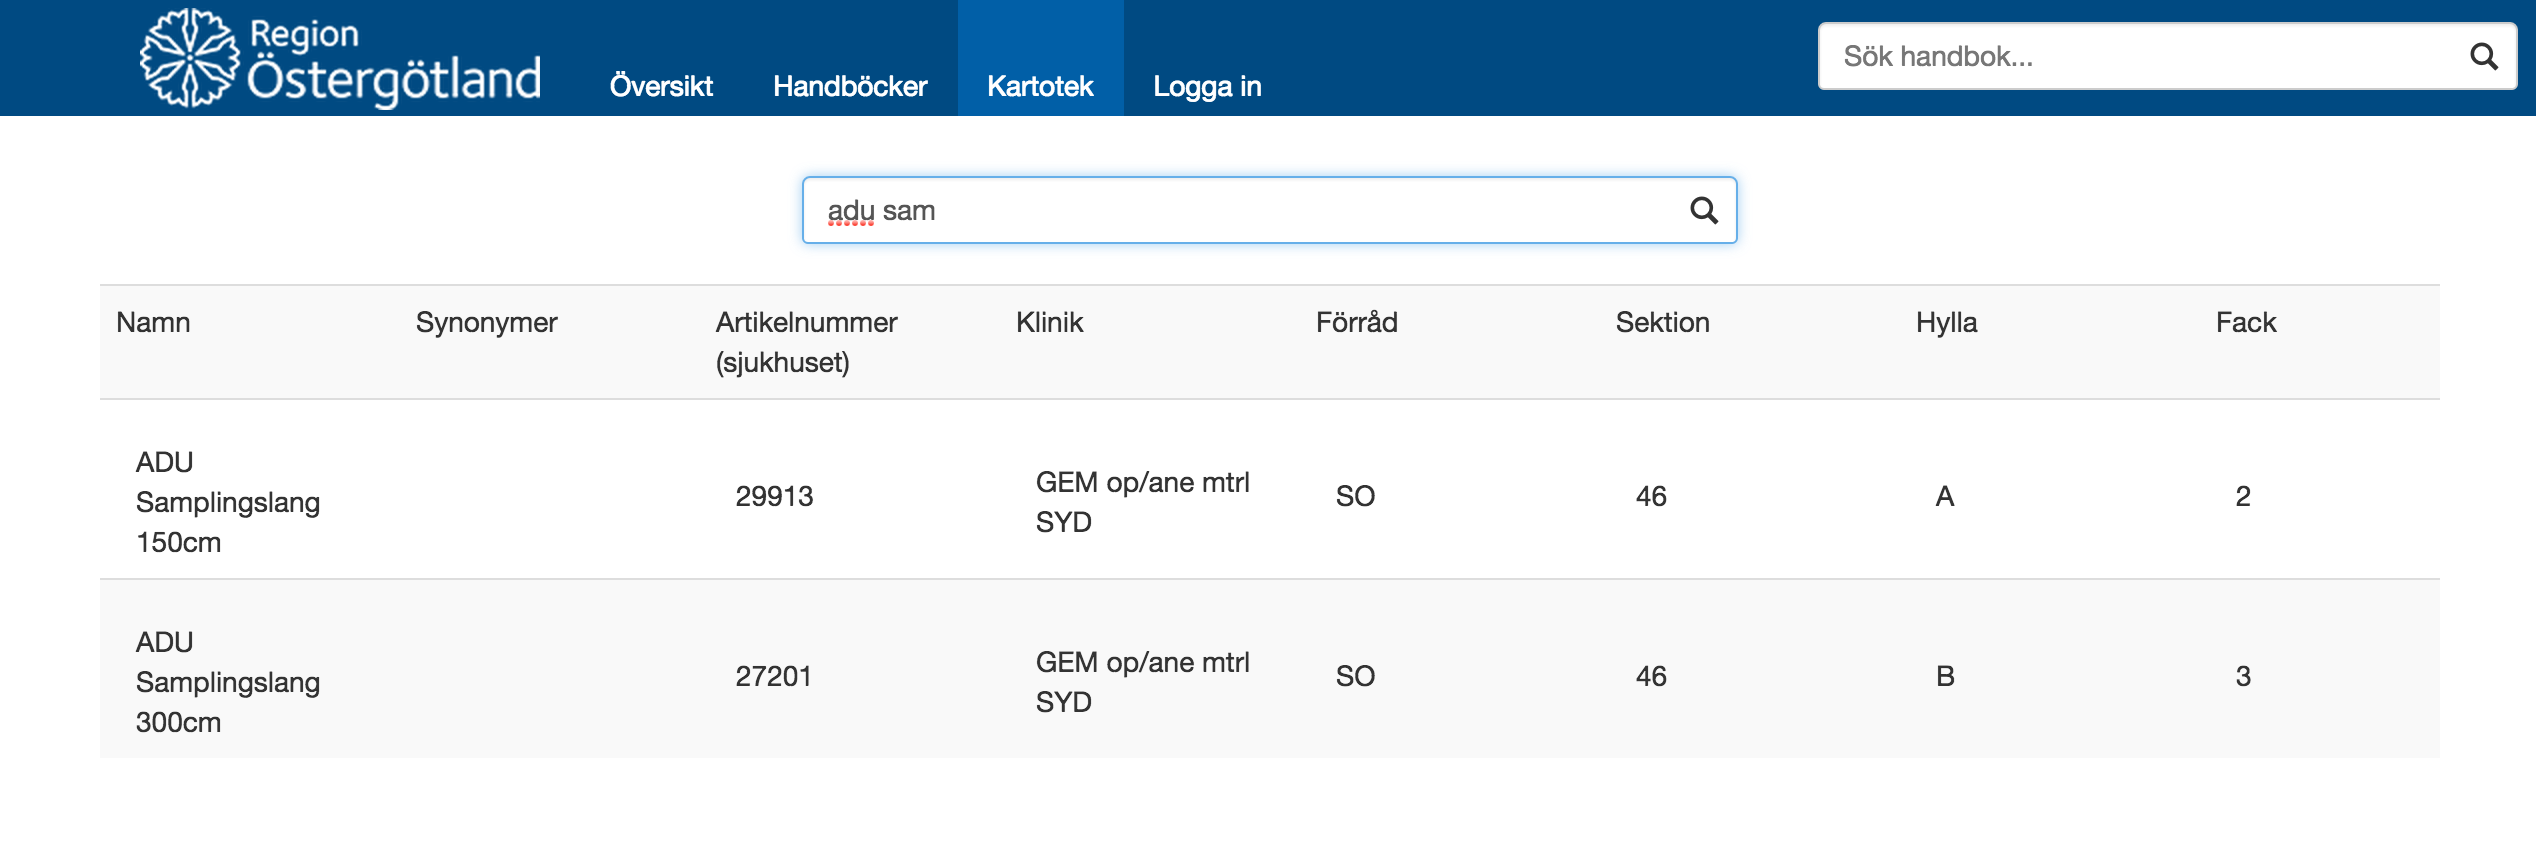
\includegraphics[width=0.9\textwidth]{images/site/kartsearch.png}
  \caption{Sökning i kartoteket.}
  \label{fig:kartsearch}
\end{figure}

Sökfunktionen är enkel.
Längst upp på sidan finns det en liten sökruta.
Användaren har möjlighet att söka på artikelnamn, artikelnummer
eller synonymer till namnet. Se ett exempel på sökning
av artikelnamn i figur \ref{fig:kartsearch}.
När man söker på någonting så byts hela tabellen ut mot sökresultatet.
Hela upplevelsen är inspirerat av "\textit{Google Instant}".

\clearpage
\subsubsection{Integrering med handböckerna}
Kartoteket står inte i isolation.
En nyckelanledning till att det är så användbart är
för att det är integrerat med handböckerna.
Det leder oss till frågeställningen:
\begin{quote}
  Går det att integrera systemet för handböcker med kartoteket utan att förlora funktionalitet?
\end{quote}
Svaret på detta anser jag vara: Ja!
Och i detta avsnitt hade jag tänkt övertyga om denna slutsats.

Integreringen sker primärt på två ställen.
\begin{enumerate}
  \item När man skapar en ny handbok.
  \item När man förbereder en operation.
\end{enumerate}

När man skapar en handbok så är kartoteket integrerat på det sättet att
när man lägger till artiklar som måste hämtas från lagret så söker man
i kartoteket för att hitta dessa. Detta är en förbättring av förra
systemet då det förut inte fanns det ingen koppling mellan dessa system.

När man förbereder en operation så är kartoteket integrerat på
så sätt att om en artikel slutar säljas, eller den av någon anledning
tas bort från kartoteket, informerar vi användaren om att den
har utgått.

Som vi har nämnt tidigare så fanns ingen av dessa av dessa funktionaliteter
förut. Eftersom vi dessutom har lyckats reproducera all funktionalitet
som fanns i det förra systemet så anser jag att frågan är klart och
tydligt positivt bekräftad.


\subsection{Diskussion}
Har vi lyckats med kartoteket? Och framför allt, är
kunden nöjd? Fick kunden de dom önskade?

Svaret är otvivelaktigt: Ja! Det finns
givetvis små buggar här och där. Ingen
produkt blir någonsin 100\% bugg-fri.
Men i våra informella intervjuer under de två studiebesök vi gjorde hos kunden
under iteration 3, där kunden har testat
vårt system en hel dag, så verkade de enormt nöjda.


%\subsubsection{Resultat}
%\subsubsection{Metod}


\subsection{Slutsatser}
Allt som allt så blev vi väldigt nöjda med kartoteket.
Det finns såklart, som alltid, saker vi skulle vilja förbättra om vi
hade mer tid, som integrering i lagret med t.ex. saldo.
Men vi anser det som finns nu, kärnfunktionaliteten,
ger en märkbar förbättring gentemot det nuvarande systemet.




\subsection{Referenser}
\vspace{-9mm}
\renewcommand{\refname}{}
\begin{thebibliography}{9}

\end{thebibliography}

\newpage
\section{Jonas Andersson}
\subsection{Inledning} 
Tidigare när jag har utvecklat webbprogram så har jag använt mig av PHP tillsammans med HTML, css och javascript. Jag har dessutom valt att skriva mycket själv och inte förlita mig på ramverk och bibliotek. I detta projekt valde jag, som arkitekt, istället att byta ut PHP mot node.js. Dessutom har jag lagt mycket vikt på använda bibliotek så mycket som möjligt för att slippa uppfinna hjulet på nytt.
\subsubsection{Syfte}
Syftet med denna del av rapporten är att analysera vad det finns för fördelar och nackdelar med att använda node.js gentemot andra vanliga språk för webben. Det ska även undersökas hur inlärningskurvan beror på språk och externa ramverk och bibliotek.
\subsubsection{Frågeställning}
Frågeställningar
\begin{itemize}
  \item Vad finns det för fördelar/nackdelar med node.js gentemot andra språk för webben?
  \item Vad finns det för fördelar/nackdelar med att använda mycket externa bibliotek?
\end{itemize}
\subsubsection{Avgränsningar}
Det finns många programmeringsspråk som man kan använda i samma syfte som node.js. Eftersom jag enbart har tidigare erfarenheter av PHP och Python så kommer node.js jämföras mot dessa och inga andra. 
\subsection{Bakgrund}
\subsection{Teori}
Node.js är en plattform för att skapa applikationer till framförallt webbservrar. Det finns en inbyggd pakethanterare vid namn npm som gör det enkelt att inkludera både små och stora bibliotek i sina projekt. Det är därför väldigt enkelt att använda sig av ett bibliotek istället för att skriva all funktionalitet själv.\\

Javascript är det programmeringsspråk som används i Node.js. På klienten, d.v.s. i webbläsaren, är man tvingad att använda sig av javascript eller något programmeringsspråk som kan kompileras till javascript. Genom att använda node.js får man därav samma språk på både server och klient. \\
\subsection{Metod}

\subsection{Resultat}
\subsection{Diskussion}
\subsubsection{Resultat}
\subsubsection{Metod}
\subsection{Slutsatser}
\subsection{Referenser}
\vspace{-9mm}
\begin{thebibliography}{9}

\end{thebibliography}
\newpage
\section{Pål Kastman}
\subsection{Inledning}
I detta projekt så har vi valt att inledningsvis skriva dokumentationen i Googles ordbehandlingsprogram Google Docs för att 
i ett senare skede då det var dags att påbörja denna rapport gå över till att använda typsättningssystemet Latex. 

Vi valde att göra på detta sätt för att så snabbt som möjligt komma igång, då man bland annat i Google Docs kan se live 
vad andra skriver.

\subsubsection{Syfte}
Syftet med denna individuella del är att undersöka funktionaliteten i Latex och väga fördelar mot nackdelar.

\subsubsection{Frågeställning}
\begin{itemize}
\item Vad finns det för begränsningar i Latex
\item Kommer det att vara en fördel eller en nackdel för flera gruppmedlemmar att jobba samtidigt i samma delar av rapporten.
\end{itemize}

\subsubsection{Avgränsningar}
Denna rapport kommer att avgränsas för att endast jämföra Latex, Microsoft Office och Google Docs, detta för att 
inte behöva jämföra alla olika ordbenhandlingsprogram.

\subsection{Bakgrund}
Dokumentering är någonting som är viktigt att göra när man arbetar i projektform, dels för egen del utifall man behöver 
gå tillbaka och se vad som gjorts, men även för andras skull ifall man kanske får en ny medarbetare som ska integreras i 
projektet. En fråga som man alltid behöver besvara är i vilket ordbehandlingsprogram dokumentationen skall skrivas. Det populäraste 
alternativet kan tänkas vara Microsoft Word, vilket har funnits sedan 1983 \cite{word_ursprung}.
\newline
Ett annat alternativ som blir allt vanligare är Google Docs, vilket är ett web-baserat ordbehandlingsprogram som lanserades av Google 2006 \cite{docs_launch} efter att man hade köpt upp företaget Upstartle \cite{upstartle}.
\newline
Ett tredje och inte lika vanligt alternativ är Latex, vilket inte är ett ordbehandlingsprogram utan istället ett märkspråk
 så som t.ex. HTML, där man istället för med ett grafiskt gränssnitt formaterar sin text,sätter sin text inom speciella taggar så att när koden senare kompileras får rätt utseende.

Latex är egentligen bara en uppsättning makron skrivna för språket Tex, vilket skapades av den amerikanske matimatikern Donald Knuth 1978 \cite{donald_knuth}. I början av 80-talet så vidareutvecklade Leslie Lamport Tex med hjälp av dess makrospråk till det som 
idag är Latex \cite{leslie_lamport}.

Vad det gäller min egen bakgrund i Latex så hade jag när detta projektet påbörjades endast använt det i ett tidigare projekt, under det projektet
blev jag dock inte så insatt i Latex utan fyllde endast i material i de redan färdiga mallarna vi hade.

Under kursens gång har jag dock skrivit en laborationsrapport i Latex och därigenom skaffat mig lite mer erfarenhet.


\subsection{Teori}
När Microsoft utvecklade Word på 80-talet så ville de naturligtvis att dåtidens datorer skulle klara av att ladda 
dokument utan att det skulle vara alltför prestandakrävande, därför konstruerade man dess filformat (.doc) binärt och gjorde konstruktionen 
väldigt komplex. Detta medförde att bara personer som var riktigt insatta i detta filformat klarade att ändra direkt i dessa filer. Google docs däremot använder sig av "molnet" för att spara filer och man behöver därför aldrig oroa sig över säkerhetskopiering. Textformatering i båda dessa program görs främst genom att använda det grafiska gränssnittet, men kan även göras genom tangentbordskommandon.
\newline
Latex är i motsats till Word och Google docs inget ordbehandlingsprogram, utan istället ett märkspråk liksom HTML. När man i Word och Google docs 
ändrar textformateringen genom ett grafiskt gränssnitt så markerar man istället sin text i Latex med taggar, som senare när man kompilerar koden ger
det önskade utseendet. Detta gör att man som användare behöver bry sig mindre om utseendet av dokumentet och kan istället fokusera på innehållet.


\subsection{Metod}
Vi har till en början valt att under projektets gång arbeta i endast en fil för den gemensamma delen av kandidatprojektet. Vad det gäller 
de individuella delarna så har vi valt att lägga dessa i separata filer och sedan importera dessa till den gemensamma. Vi 
sparar alla dokumentfiler i samma repository på github som vi har källkoden.

Genom att göra på detta sätt så kan vi garantera att det inte kommer att uppstå några konflikter i de individuella delarna.
Det som vi inte vet, är huruvuda det kommer att uppstå problem då alla gruppmedlemmar skall skriva på den gemensamma delen.

\subsection{Resultat}
\subsection{Diskussion}
\subsubsection{Resultat}
\subsubsection{Metod}
\subsection{Slutsatser}
\subsection{Referenser}
\begin{thebibliography}{9}
\bibitem{word_ursprung}
\url{http://ia801406.us.archive.org/21/items/A\_History\_of\_the\_Personal\_Computer/eBook12.pdf}.\\
 Sida 11-12. Hämtad 2015-04-20.

\bibitem{docs_launch}
\url{http://googlepress.blogspot.se/2006/06/google-announces-limited-test-on-google_06.html}.\\
 Hämtad 2015-04-28.

\bibitem{upstartle}
\url{http://googleblog.blogspot.se/2006/03/writely-so.html}.\\
 Hämtad 2015-04-28. 

\bibitem{donald_knuth}
\url{https://gcc.gnu.org/ml/java/1999-q2/msg00419.html}.\\
 Hämtad 2015-04-20.

\bibitem{leslie_lamport}
\url{http://research.microsoft.com/en-us/um/people/lamport/pubs/pubs.html#latex}.\\
 Hämtad 2015-04-20.

\end{thebibliography}

\newpage
\section{Kravinsamlingsmetoder - Daniel Falk}
\subsection{Inledning}
Jag har i detta projekt haft rollen som analysansvarig vilket innebär en analys av kundens behov och framställning av krav utifrån dessa. Denna enskilda del beskriver vilka kravinsamlingsmetoder och verktyg som använts för att ta fram krav. Erfarenheterna används för att undersöka om metoderna och verktygen kan användas för att tillfredsställa kundens verkliga behov.
\subsubsection{Syfte}
Syftet med denna del av rapporten är att undersöka olika metoder och verktyg för kravframställning. Fokus ligger på intervjuer, observationer och prototyper. Rapporten går speciellt in på hur prototyper använts för att ta fram, testa och validera krav i detta projekt.
\subsubsection{Frågeställning}
%Hur kan man samla in krav som tillfredställer kundens verkliga behov?
\begin{itemize}
\item Är intervjuer och observationer bra metoder för att analysera kundens behov?
%\item Hur kan intervjuer och observationer användas för att analysera kundens behov?
\item Hur kan man arbeta med prototyper för att framställa krav?
\item Hur kan man använda prototyper för att testa och validera krav?
\end{itemize}
\subsubsection{Avgränsningar}
Rapporten har sin utgångspunkt i hur kravframställningen gått till i detta projekt och gör inga jämförelser med andra kravinsamlingsmetoder. Metoden bör inte ses som ett allmänt tillvägagångssätt.
\subsection{Bakgrund}
Att förstå kundens verkliga behov utgör grunden för ett lyckat projekt. Ett projekt faller ofta på grund av ofullständiga krav \cite{Hull}.
För att samla in krav kan flera olika metoder och tekniker användas. Metoderna kan variera och vara olika bra på att fånga upp olika typer av krav.
\subsection{Teori}
Teorin beskriver kravinsamlingsmetoder och  verktyg som använts i detta projekt. %och vilka problem som kan uppstå vid kravframställning. 
%\subsubsection{Problem}
%Skriv om och flytta till bakgrund
%Det finns ett antal barriärer som kan uppstå vid kravframställning. Ett problem är ofta att kunden inte kan formulera vad de vill ha. De kan se problemet men inte vad som behöver göras. De kan överdriva vissa problem medan andra förbises. 
%Ett annat problem är att kunden kan ha fastnat i ett invant mönster. De kan ha svårt att föreställa sig nya sätt att utföra en uppgift på.
%\cite{Lauesen} %Kolla upp om denna parafras är ok.

\subsubsection{Prototyper}
Prototyp är ett ord som har sina rötter i grekiskan och betyder \textit{första form} \cite{Arvola}. Deras syfte är att i ett tidigt skede beskriva hur det färdiga systemet ska fungera. Prototyper kan användas för att testa olika ideér och designer och kan variera i detaljrikedom. 

En tydlig skillnad är den mellan enkla LoFi-prototyper skissade på papper och datorbaserade HiFi-prototyper som mer liknar det riktiga systemet. LoFi-prototyper är ett bra verktyg för att snabbt kunna diskutera ett designval då det kräver väldigt lite arbete. En styrka hos LoFi-prototyper är att användare har lätt att komma med kritiska kommentarer utan att känna att de förolämpar designern \cite{Arvola}.

Prototyper kan vara temporära eller evolutionära \cite{Arvola}. En temporär prototyp är en prototyp som slängs efter att man har använt den och utvärderat den. En evolutionär prototyp slängs inte utan byggs vidare på. Man kan se det som en tidig version av det slutgiltiga systemet. En sådan prototyp kan användas i en livscykelmodell för att samla in krav \cite{Dorfman}. I modellen itereras kravinsamling, prototypdesign, kodning och testning av prototypen.

\subsubsection{Intervjuer}
%För att samla in krav kan flera olika metoder och tekniker användas. Metoderna kan variera och vara olika bra på att fånga upp olika typer av krav.
Intervjuer är en bra teknik för att få information om det nuvarande arbetet inom området och problem relaterade till det. Det är också bra för att få fram de stora målen med ett projekt. Många ser det som den huvudsakliga insamlingstekniken. De ger mycket information men för att lösa kritiska problem behövs ofta andra tekniker för att komplettera intervjuer \cite{Lauesen}. 
\subsubsection{Observationer}
Observationer är ett bra verktyg för att få information om nuvarande system eller arbetssätt. Det är ett bra sätt att komplettera intervjuer då användare ofta har svårt att förklara vad de verkligen gör \cite{Lauesen}. 
%(task demonstration)
%(scenarios)
 
\subsection{Metod}
Denna del beskriver hur intervjuer, observationer och prototyper har använts som metoder för kravframställning i detta projekt. Metoden beskriver också hur systemet testats för att validera och testa kraven. Frågeställningarna besvaras utifrån denna erfarenhet.
%Denna del beskriver hur kravframställningen gått till i detta projekt. Först beskrivs arbetet med att analysera kundens behov under förstudien. Vidare beskrivs mer ingående vilka metoder som använts och hur kraven valdes att representeras. Avslutningsvis beskrivs vilka användartester som genomfördes och hur dessa bedrog till utvecklingen.
%\subsubsection{Förstudie}
%Den största delen utav analysarbetet skedde under förstudien. Här identifierades de olika intressenterna och en kravspecifikation utarbetades. Våran första kontakt med projektet var en projektbeskrivning där kunden formulerade sina mål och visioner av projektet. Några vikta krav gavs också såsom att prototypdesign skulle genomföras i samarbete med kunden. Ett första möte utav fyra under förstudien gav sedan mer information och vi började våran kravinsamling. Vi kunde konstatera att vi hade två olika intressenter att arbeta med. Dels sjuksköterskorna som är användare av systemet och dels CMIT, Centrum för medicinsk teknik och IT, som ansvarar för sjukhusets IT-miljöer. För att förstå användarnas behov hölls ett studiebesök där vi fick en visning av nuvarande system och hur det används. Detta var nödvändigt för att verkligen förstå vad det var som behövde göras och vad som kunde förbättras. Från CMIT:s sida hölls mer tekniska möten där teknikval diskuterades. Här var det viktigt att ta reda på vilka begränsningar som fanns och vilka val som passade våra och deras erfarenheter.
\subsubsection{Intervjuer}
Möten med kund har genomförts vilka kan ses som intervjuer. Dessa möten har skett dels med IT-ansvariga, verksamhetsutvecklare och sjuksköterskor. För att samla in krav under dessa möten har vi dels fört anteckningar på papper eller dator och dels spelat in på mobil. När vi varit flera personer på möten har vi gått igenom och diskuterat våra anteckningar i efterhand. Vid oklarheter har vi antecknat dessa för att förtydliga med kund. Inspelning användes främst vid första mötet och var användbart då vi fick mycket information att sätta oss in i. 
%Kravspecifikationen skrev i Google docs. Detta valdes eftersom kraven utarbetades tillsammans med kund. Ett gemensamt redigerbart dokument gav en möjlighet för oss att arbeta på olika platser under kravframställningen vilket var effektivt. En kommentarsfunktion gav oss möjligheten att kommentera krav och föreslå förbättringar. Under interna möten och kundmöten var den gemensamma redigeringen också till nytta då kravformuleringar snabbt kunde genomföras.

%\subsubsection{Kravrepresentation}
%Kraven gavs en prioritetsordning för att kunna urskilja de mest väsentliga kraven. Detta kändes nödvändigt då vi var begränsade av en tidsbudget. En prioritering av kraven gav utrymme för vidareutveckling i mån av tid. Krav med prioritet 1 var att betrakta som grundkrav som skulle genomföras för att projektet skulle ses som godkänt. Krav med prioritet 2 var att betrakta som önskvärda och som skulle genomföras om då grundkraven var genomförda. Krav med prioritet 3 var krav som fångats upp med som skulle ses som framtida utbyggnad. 
%Koppla till nån litteratur/standard.

%Strukturering av krav
%Kraven numrerades för att lätt kunna refereras till under projektets gång. De delades också in i olika sektioner efter deras del i systemet. Sektionerna var plocklistor, handböcker, kartotek, lagersystem. En extra sektion för generella krav användes. Denna uppdelning kändes naturlig för detta projekt. 
%Man skulle också kunna dela in dem efter blablabla...

%Kravspecifikationen skrevs med stöd från standarden IEEE 830. Enligt standarden ska ett krav vara korrekt, otvetydigt, färdigt, konsekvent, prioriterat, verifierbart, modifierbart och spårbart. Detta eftersträvades men det kan diskuteras om alla krav passerar dessa filter. I slutändan var det ändå våran gemensamma förståelse för kravet tillsammans med kunden som accepterades. 

%Enligt standarden uttrycktes kraven på ska-form. Ett exempel på ett krav från projektet är följande: "Plocklistor ska innehålla information om artikelns namn, förråd, sektion, hylla och fack".

\subsubsection{Observationer}
För att få en inblick i hur operationsförberedelserna fungerar i dagsläget genomfördes ett studiebesök på sjukhusets operationsavdelning. Vi fick här se problemet ur sjuksköterskornas synvinkel. Vi fick se hur man arbetade i artikellagret i dagsläget vilket var nödvändigt för att kunna genomföra en förbättring. De svårigheter som beskrivits blev tydligare och det blev lättare att föreställa sig en lösning på problemet.

\subsubsection{LoFi-prototyper}
Under förstudien valde vi att vid två tillfällen göra LoFi-prototyper som vi tog med till kund. Vid dessa tester kunde vi se om vi var på rätt bana när det gällde design och struktur. LoFi-prototyperna utgjordes av enkla pappersskisser. Ett exempel visas i figur~\ref{fig:lofiprototyper}.
\begin{figure}[htbp]
\begin{center}
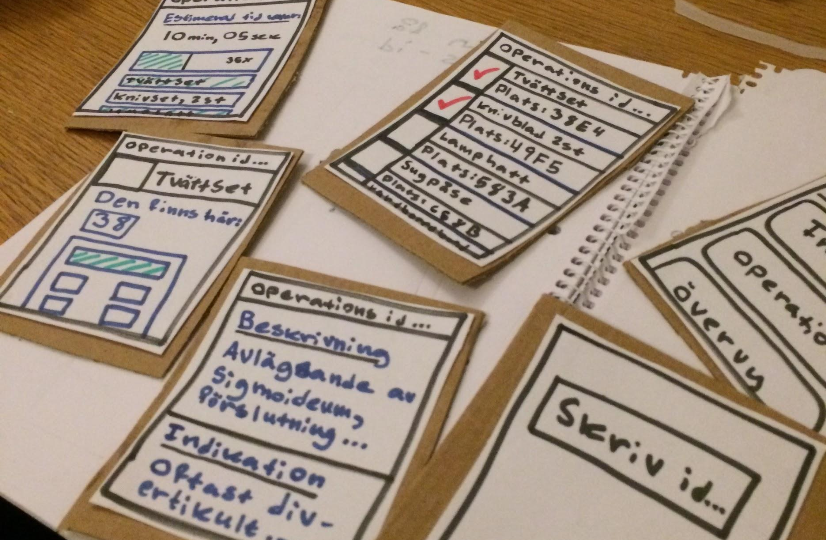
\includegraphics[scale=0.2]{lofiprototyper.png}
\caption{LoFi-prototyper}
\label{fig:lofiprototyper}
\end{center}
\end{figure}

Det första tillfället fokuserade på gränssnittsdesign och navigation i systemet. Prototyperna visades för en sjuksköterska som fick föreställa sig systemet. De olika korten gicks igenom för att se om vi hade hittat en bra design och om navigationen var logisk.

Vid det andra tillfället hade vi en intern brainstorming för att ta fram en design för redigeringsvyn av en handbok. Två olika förslag togs fram och presenterades för kunden. Vi observerade och antecknade försökspersonernas olika tankar samt spelade in en ljudupptagning på mobiltelefon för att kunna gå tillbaka och analysera.
%Note to self: Lyssna på det ljudklippet.
\subsubsection{HiFi-prototyp}
Själva systemet som vi utvecklat kan ses som en HiFi-prototyp. Den är evolutionär på så sätt att den byggts vidare på under varje iteration. Huruvida kunden kommer fortsätta utvecklingen av denna prototyp på egen hand är inte bestämt. Ett alternativ är att se vårt system som en prototyp till ett nytt system. 
Prototypen presenterades och utvärderades i samband med kundmöten vid varje iterationsslut. Ett mer omfattande användartest utfördes i iteration 3.


%\subsubsection{Kravvalidering}
%Vid varje iterationsslut hölls ett möte med kund där vi demonstrerade nya features och lät kunden testa systemet. Iterationerna gjorde att vi snabbt kunde rätta till eventuella missförstånd. Vid dessa möten diskuterade vi också vad som skulle genomföras nästa iteration. Vi gick igenom vilka krav som var genomförda och vilka som skulle prioriteras till nästa iteration.

\subsubsection{Användartest}
I iteration 3 av projektet genomfördes användartester av systemet vid två tillfällen. Vid dessa tester kördes det nya systemet parallellt med det gamla. Testen fokuserade på skapande av handböcker och genomförande av operationsförberedelser. Testen genomfördes dels på egen hand av verksamheten och dels med delar av projektgruppen på plats. Vid användartesterna fick vi in feedback från användarna om vad som var bra och vad som kunde göras bättre. Ett exempel på designval som kunde utredas vid testningen var om en operationsförberedelse skulle kunna sättas som klar även om inte alla artiklar var plockade. Olika alternativ hade diskuterats innan men vid testning blev det tydligt att det var en önskvärd funktionalitet. Andra exempel på saker som upptäcktes vid användartesten var hur engångsmaterialet skulle sorteras på bästa sett,hur navigationen mellan olika sidor kunde fungera effektivare och att vissa saker inte användes.
Systembuggar kunde också rapporteras och åtgärdas under testningen.
Kunden höll också en intern utvärdering om hur användarna upplevde systemet (se Appendix A).

%skriv eventuellt om de övriga artiklarna som inte behandlas under engångsmaterial

\subsection{Resultat}
Att använda intervjuer och observationer som metoder för kravinsamling kändes naturligt för detta projekt. Det var ett bra tillvägagångssätt för att få en helhetsbild av vad kunden ville ha. Intervjuerna gav oss kundens mål och visioner av projektet. Observationerna gav oss en inblick i hur användarna använde systemet och saker som var otydliga i intervjuerna kunde fångas in i observationen. På så sett kompletterade dessa metoder varandra och det kändes nödvändigt för en lyckad kravinsamling.

LoFi-Prototyper kunde användas i förstudien för att bekräfta våran bild av vad som skulle byggas. De var ett bra verktyg för att reda ut otydligheter. De var effektiva på så sätt att de gick snabbt att tillverka och gav mycket feedback tillbaks. Det kändes lättare att diskutera systemet när vi hade något visuellt framför oss. De gjorde det lättare att formulera krav och bidrog på så sätt till kravinsamlingen.

HiFi-prototypen kunde användas för att testa systemet utifrån kraven. Vid varje iterationsmöte kunde systemet utvärderas och kraven kunde både formuleras om och prioriteras om. Vi kunde också använda prototypen för att validera vilka krav som var genomförda. 
 
Vid användartesterna i iteration 3 kunde systemet användas för att testa om kraven uppfyllts och formulerats efter kundens behov. Här framkom vissa förändring på krav såsom att mer information skulle visas för en artikel. Prototypen kunde på så sätt användas för att testa och validera krav. För en eventuell vidareutveckling kan observationerna användas som underlag för att skriva nya krav.
%TODO: Fyll på med resultat från användarutvärdering

\subsection{Diskussion}
Här diskuteras resultatet av den enskilda utredningen och hur metoden fungerat för att undersöka frågeställningarna.
\subsubsection{Resultat}
Resultatet bekräftar synen på vad som sägs i teorin. Intervjuer och observationer kunde användas som komplement till varandra på ett bra sätt. Det kan diskuteras om dessa metoder är tillräckliga för en kravinsamling. För ett projekt i en storlek som vårt kan de vara tillräckliga. 

Prototyper användes i vårt projekt som ett verktyg för att samla in krav. Andra verktyg kunde dock ha använts för att ytterligare komplettera dessa metoder. 

Vi la inte så stort fokus på systemets olika roller i projektet utan nöjde oss med två stycken. För att analysera de olika rollerna kunde verktyg som user-stories ha använts.
Prototyper kan se olika ut och användas på många olika sätt. I vårt projekt visades att de var bra för att samla in krav och snabbt reda ut otydligheter. 
\subsubsection{Metod}
Metoden som användes för att svara på frågeställningarna var att utföra själva projektet och utgå ifrån dessa erfarenheter. Projektet gav således svar på att intervjuer, observationer och prototyper gick att använda och var bra för just detta projekt. Metoden har inte gjort några jämförelser till andra kravinsamlingsmetoder vilket skulle kunna vara intressant. 
%Huruvida metoden passar andra projekt kan diskuteras. 

\subsection{Slutsatser}
Intervjuer och observationer är bra grundmetoder för att analysera kundens behov. I detta projekt kändes de som naturliga och nödvändiga tillvägagångssätt. De kan med fördel kompletteras med olika verktyg och tekniker såsom prototyper. 

Prototyper är ett väldigt kraftfullt verktyg för kravinsamling och kan användas på flera olika sätt. LoFi-prototyper är bra i början av ett projekt för att snabbt kunna kommunicera ideér och hitta en bra design. De hjälper på så sätt till i kravinsamlingsprocessen. HiFi-prototyper är bra både för att testa om kraven formulerats på ett bra sätt och för att validera systemets funktionalitet.
%\subsection{Referenser}

%Note to self:Dubbelkolla referenserna, tror det är fel standard
%\vspace{-9mm}
%\begin{thebibliography}{9}

%\bibitem{Hull}
%Hull. E, Ken. J och Jeremy. D, Requirements Engineering, Third edition. London: Springer, 2011.

%\bibitem{Arvola}
%Arvola, M. (2014) Interaktionsdesign och UX: Om att skapa en god användarupplevelse. Studentlitteratur AB, Lund.

%\bibitem{Dorfman}
%Dorfman, M. (1997) Requirements Engineering. Institute of Electrical and Electronics Engineers, Inc. 

%\bibitem{Lauesen}
%Lauesen, S. (2002) Software Requirements: Styles and Techniques. Harlow: AddisonWessly.

%\end{thebibliography}


\newpage
\section{Automatiserade tester med Travis CI - Erik Malmberg}
\subsection{Inledning}
Den här enskilda utredningen är en del av kandidatrapporten i kursen TDDD77 vid Linköpings universitet.
Utredningen behandlar en del av utvecklingen av ett webb-baserat system för att underlätta förberedelser
inför operationer på sjukhusen i Östergötland. Systemet utvecklades på uppdrag av Region Östergötland.

\subsubsection{Syfte}
Syftet med den här enskilda delen av kandidatarbetet är att ge insikt i hur kontinuerlig integration och 
automatiserade tester kan användas för att effektivisera testandet i ett projekt som använder en agil 
utvecklingsmetod. Speciellt ska det undersökas hur väl det går att använda Travis CI tillsammans med 
ramverket Jasmine.

\subsubsection{Frågeställning}
De frågeställningar som ska besvaras i den här enskilda delen av rapporten är:

\begin{itemize}
\item Hur kan man använda Travis CI tillsammans med Jasmine för att testa en 
webbapplikation byggd på javascript och node.js?
\item Hur många tester hinner Travis CI köra på en sekund?
\item Vilka typer av tester är svåra att utföra?
\end{itemize}

I svaret på den andra frågeställningen ska testfallen specifieras noggrant 
så att svaret inte blir tvetydigt.

\subsubsection{Avgränsningar}
Inga undersökningar kommer att utföras om hur andra lösningar än Travis CI kan användas för kontinuerlig 
integration. De testfall som kommer användas kommer uteslutande att vara skrivna med ramverket Jasmine.

\subsection{Teori}
Här beskrivs den teori som är nödvändig för att förstå rapporten.

\subsubsection{Vattenfallsmodellen}
I vattenfallsmodellen genomförs all integration och alla tester efter att implementeringen är slutförd. 
Om ett problem då identifieras under integrationen så är det krångligt att gå 
tillbaka och åtgärda problemet. 
Det kan leda till förseningar av projektet.
Om felet som upptäcks är så allvarligt att en betydande omdesign måste ske så
kommer utvecklingen i stort sett att börja om från början och man kan räkna 
med en hundraprocentig ökning av budgeten, 
både vad gäller pengar och tid \cite{Royce}.

\subsubsection{Kontinuerlig integration och automatiserade tester}
Kontinuerlig integration kan leda till att problemen identifieras tidigare i 
utvecklingsprocessen. Problemen blir då lättare att åtgärda. Automatiserade tester kan effektivisera 
testprocessen och det finns många tillgängliga lösningar för att köra automatiserade
tester \cite{Karlsson}.
Några av de vanligaste är Travis CI, Codeship och Drone.

\subsubsection{Travis CI}
Travis CI är en webb-baserad tjänst för att köra automatiserade enhetstester och integrationstester
på projekt som finns på GitHub. Travis CI är byggt på öppen källkod och är gratis att använda. 
Tjänsten har stöd för många olika programmeringsspråk, men det som är 
relevant för innehållet i den här rapporten
är javascript med node.js. För att konfigurera Travis CI används filen .travis.yml 
som placeras i det aktuella
projektets repository på GitHub.

\subsubsection{Javascript}
Javascript är ett programmeringsspråk som i första hand används på klientsidan på webbsidor.
Javascript exekveras av webbläsaren och arbetar mot ett gränssnitt som heter 
Document Object Model (DOM).

\subsubsection{JQuery}
JQuery är ett javascript-bibliotek som kan användas för att förenkla programeringen
av javascript på klientsidan av en webbsida. JQuery innehåller lättanvänd
funktionalitet för händelsehantering och modifiering av HTML-objekt.
JQuery är gratis och baserat på öppen källkod som är tillgänglig under en
MIT-licens.

\subsubsection{Node.js}
Node.js är en runtime environment för internetapplikationer. Det kan till exempel 
användas för att skapa webbservrar.
Node.js är baserat på öppen källkod och det är enkelt att lägga till nya 
moduler för att anpassa det system man vill
använda. För att lägga till nya moduler används node package manager (npm).

\subsubsection{Jasmine}
Jasmine är ett ramverk för testning av Javascript. 
Den node-modul som används är grunt-contrib-jasmine som använder task runnern Grunt 
för att köra testfall som skrivits med Jasmine.
Grunt kunfigureras med filen Gruntfile.js.

\subsection{Metod}
Arbetet inleddes genom att Travis CI kopplades till projektets repository på GitHub.
Kopplingen utfördes
genom att administratören för repositoryn loggade in på travis-ci.org med 
sitt GitHub-konto och aktiverade
en webhook för repositoryn.\\

Inställningarna för Travis CI konfigurerades med filen .travis.yml i projektets
repository. Språket valdes till
javascript med node.js med inställningen: \emph{language: node\textunderscore js}.
Versionen av node.js valdes till version 0.10
med inställningen: \emph{node\textunderscore js: "0.10"}.\\

De nödvändiga node-modulerna installerades med hjälp av node package manager (npm).
Grunt installerades
med kommandot: \emph{npm install -g grunt-cli}. Grunt-contrib-jasmine installerades med kommandot: 
\emph{npm install grunt-contrib-jasmine}.\\

Task runnern Grunt konfigurerades med filen Gruntfile.js i projektets repository.
En task för Jasmine laddedes in med
inställningen: \emph{grunt.loadNpmTasks('grunt-contrib-jasmine');}.
Tasken konfigurerades med följande kod i Gruntfile.js.

\begin{lstlisting}[
  basicstyle = \small
]
module.exports = function(grunt) {

  grunt.initConfig({
    pkg: grunt.file.readJSON('package.json'),
    jasmine: {
      test: {
        src: './public/js/*.js',
	options: {
	  vendor: [
	    'public/js/lib/jquery/jquery-2.1.1.js',
	    'node_modules/jasmine-jquery/lib/jasmine-jquery.js'
          ],
	  keepRunner: true,
	  specs: 'test/*-spec.js',
	  template: 'test/template/spec-template.tmpl'
        }
      }
    }
  });

  grunt.loadNpmTasks('grunt-contrib-jasmine');
}
\end{lstlisting}

Med \emph{src: './public/js/*.js'} valdes de filer som som skulle testas.
Med vendor valdes andra filer som var nödvändiga för att köra testerna.
Raden \emph{keepRunner: true} gör att filen \textunderscore SpecRunner.html sparas efter att
testerna körts. Filen kan sedan öppnas i en webbläsare och innehåller
detaljerad information om utfallet av testerna.
Med \emph{specs: 'test/*-spec.js'} valdes de testfall som skulle köras.
Alla filer som slutar med -spec.js i mappen test anses alltså vara
testfall som ska köras.
Raden \emph{template: 'test/template/spec-template.tmpl'i} gör att testerna
körs med en speciell SpecRunner som även kan innehålla HTML som testfallen
kan modifiera.
Eftersom Travis CI använder npm för att starta 
testerna så definierades testskriptet för npm med raden
\emph{''test'': ''grunt jasmine --verbose''} i filen package.json 
i projektets repository.\\

Testfallen skrevs med Jasmine. Jasmine har en enkel och intuitiv syntax.
Ett exempel på ett testfall skrivet med Jasmine följer nedan.

\begin{lstlisting}[
  basicstyle = \small
]
describe('The function splitOnce', function() {
	
  it('can split a string with a char correctly', function() {
    var str = 'a.b.c.d';
    var res = splitOnce(str, '.');
    expect(res[0]).toBe('a');
    expect(res[1]).toBe('b.c.d');
  });
}
\end{lstlisting}

På den första raden beskrivs vilken del av koden det är som ska testas.
På nästa rad beskrivs vad det är som ska testas i den utvalde delen av koden.
Med functionen expect kontrolleras att koden har utfört testet på det sätt
som förväntats. Flera expect-funktioner kan användas i samma testfall.\\

Ett speciellt testfall skrevs
för att besvara den andra frågeställningen om hur många tester som 
Travis CI kan köra
på en sekund. Det speciella testfallet visas nedan.

\begin{lstlisting}[
  basicstyle = \small
]
describe('Travis CI', function() {
	
  it('can do a lot of tests', function() {
    var date = new Date();
    var startTime = date.getTime();
    var time = startTime;
    var i = 0;

    while (time < startTime + 1000) {  
      var str = 'a.b.c.d';
      var res = splitOnce(str, '.');
      expect(res[0]).toBe('a');
      expect(res[1]).toBe('b.c.d');

      i++;
      date = new Date(); 
      time = date.getTime();
    };

    console.log(i);
  });
});
\end{lstlisting}

Testfallet testar funktionen splitOnce() så många gånger som möjligt
under en sekund. Antalet gånger som funktionen hann köras skrivs
sedan ut på skärmen med en console.log(). 
Testfallet har körts flera gånger på olika datum och olika tidpunkter.
Resultatet av testerna presenteras i en tabell under rubriken Resultat.
För att antalet ska
få en konkret betydelse visas även funktionen splitOnce() nedan.

\begin{lstlisting}[
  basicstyle = \small
]
var splitOnce = function(str, split) {
  var index = str.indexOf(split);
  if (index === -1) {
    return [str, ''];
  }

  return [str.slice(0,index), str.slice(index + 1)];
};
\end{lstlisting}

Funktionen tar två paramterar. En sträng (str) som ska delas upp och 
en sträng (split) som anger vilket tecken eller vilken teckenkombination
som ska dela upp strängen. Funktionen delar endast upp strängen i två delar
även om (split) förekommer påflera positioner i (str). Funktionen returnerar 
en array med två element.
De två elementen är de två delarna av den ursprungliga strängen. Om den andra
parametern (split) inte existerar i den första parametern (str) så returneras
hela strängen i det första elementet och en tom sträng i det andra elementet.\\

För att besvara den tredje frågeställningen om vilka tester som är svåra att
utföra så gicks koden igenom och försök till att skriva testfall genomfördes
med de olika delarna av koden. Resultatet av dessa tester redovisas under 
avsnittet Resultat.

\subsection{Resultat}
Här presenteras resultatet av rapporten, det vill säga svaren på
frågeställningarna.

\subsubsection{Hur kan man använda Travis CI tillsammans med Jasmine 
för att testa en webbapplikation byggd på javascript och node.js?}
Travis CI kan användas tillsammans med Jasmine för att testa en
webbapllikation byggd på javascript och node.js på det sätt som beskrivits
under avsnittet Metod.

\subsubsection{Hur många tester hinner Travis CI köra på en sekund?}
Resultatet av testerna som utfördes för att besvara den andra frågeställningen
visas i tabellen nedan.

\begin{center}
  \begin{tabular}{| l | l | l | l |}
  \hline
  Testnummer & Datum (ÅÅ-MM-DD) & Tid (hh-mm-ss) & Test per sekund\\ \hline
  1 & 15-05-01 & 13:53:34 & 11380\\ \hline
  2 & 15-05-01 & 14:27:27 & 12462\\ \hline
  3 & 15-05-01 & 14:47:14 & 9386\\ \hline 
  4 & 15-05-03 & 10:21:57 & 14093\\ \hline 
  5 & 15-05-03 & 15:43:20 & 9875\\ \hline 
  6 & 15-05-04 & 09:42:39 & 10156\\ \hline 
  7 & 15-05-04 & 11:14:43 & 11933\\ \hline 
  8 & 15-05-04 & 17:42:34 & 10056\\ \hline 
  9 & 15-05-05 & 08:32:15 & 12216\\ \hline 
  10 & 15-05-05 & 08:55:02 & 9767\\ \hline 
  11 & 15-05-05 & 09:15:16 & 10153\\ \hline 
  12 & 15-05-05 & 10:12:57 & 6992\\ \hline 
  \end{tabular}
\end{center}

Medelvärdet är:

\subsubsection{Vilka typer av tester är svåra att utföra?}
Det visade sig att vanliga javascript-funktioner är lätta
att testa så länge de ligger utanför JQuery-funktionen
\emph{\$(document).ready()}. Det kan illustreras med några
rader kod.

\begin{lstlisting}[
  basicstyle = \small
]
function easyToTest() {
  return 0;
}

$(document).ready(function() {

  $('#id1').click(
    var test = easyToTest(); 
  );

  $('#id2').click(
    //Hard to test
    var test = 0; 
  );
});

\end{lstlisting}

Det är alltså rekomenderat att skriva alla javascript-funktioner utanför 
JQuery-funktionen \emph{\$(document).ready()} eftersom koden då blir 
lättare att testa.\\

JQuery-funktioner är i allmänhet svårare att testa än vanliga
javascript-funktioner.

\subsection{Diskussion}
\subsubsection{Resultat}
\subsubsection{Metod}
\subsection{Slutsatser}
\subsection{Referenser}
\vspace{-9mm}
\renewcommand{\refname}{}
\begin{thebibliography}{9}

\bibitem{Royce}
W.W. Royce, ''Managing the development of large software systems,''
\textit{Proceedings of IEEE WESCON}, pp. 2, aug, 1970.
[Online].
Tillgänglig (nytryckt med annan sidnumrering):
\url{http://www.cs.umd.edu/class/spring2003/cmsc838p/Process/waterfall.pdf}.
[Hämtad april 28, 2015].

\bibitem{Karlsson}
O. Karlsson, ''Automatiserad testning av webbapplikationer,''
Linköpings univ., Linköping, Sverige, 2014, pp. 43.
[Online]. 
Tillgänglig: 
\url{http://www.diva-portal.org/smash/get/diva2:727654/FULLTEXT01.pdf}.
[Hämtad april 19, 2015].

\end{thebibliography}

\newpage
\section{Checkning av checklistor - Robin Andersson}
\subsection{Inledning}
Vårt system ska innehålla två olika typer av checklistor på olika webbsidor. Om flera användare är inne på samma sida samtidigt och en person checkar en checkruta så ska den checkrutan bli checkad för alla användare som är inne på den webbsidan.\\

Den ena typen av checklista är en plocklista där det finns information om vilka engångsmatrial som behövs för den operationsförberedelse som användaren är inne på samt vart de matrialen kan hämtas någonstans. När en sjuksköterska har plockat en artikel så checkar denne av den artikeln i plocklistan.\\

Den andra typen av checklista är en lista av operationssalsförberedelser där det kan stå en längre beskrivning om vad som ska göras och när en sjuksköterska har utfört hela den förberedelsen så checkar denne av den förberedelsen i förberedelselistan.

Checklistorna kommer att implementeras med hjälp av handlebars, javascript, jquery samt Socket.IO. För information om dessa språk/paket hänvisar jag till bakgrunden i den gemensamma rapporten.

\subsubsection{Syfte}
Syftet med denna del av projektet är att flera sjuksköterskor samtidigt ska kunna förbereda operationer genom att plocka olika artiklar samt förbereda operationssalen och checka av det som är utfört utan att det ska bli några konflikter med att flera sjuksköterskor plockar samma artikel eller liknande.

\subsubsection{Frågeställning}
\begin{itemize}
\item Går det att anpassa checklistan för en surfplatta medan den samtidigt innehåller information om var artiklar befinner sig samt hur många av varje artikel som behövs?

\item Kommer Socket.IO vara tillräckligt snabbt för att flera personer ska kunna checka av artiklar samtidigt utan förvirring?
\end{itemize}

\subsubsection{Avgränsningar}
Eftersom denna del av projektet endast innehåller checkande av checklistor så saknas etiska aspekter.

\pagebreak
\subsection{Teori}
\subsubsection{Websockets}
WebSockets består av ett nätverksprotokoll och ett API som gör det möjligt att skapa en WebSocket uppkoppling mellan en klient och en server. Med hjälp av WebSocket API:t så kan man hantera en full-duplex kanal som kan användas till att skicka och ta emot meddelanden. En WebSocket anslutning skapas genom att gå över från HTTP protokollet till WebSockets nätverksprotokoll när en initial handskakning mellan server och klient sker. När en WebSocket anslutning finns uppkopplad så kan WebSocket meddelanden skickas fram och tillbaka mellan metoderna som finns definierade i WebSockets gränssnitt. När WebSockets används i ett system så används asynkrona eventlyssnare för att lyssna på kommunikationen. WebSockets API är rent eventbaserat villket betyder att klienter inte behöver kontrollera om servern har uppdaterats utan att de istället uppdaterar när de får ett event. \cite{websocketbook} \\

Kanalen som WebSocket använder sig av kommunicerar över nätet med hjälp av en enda socket. WebSockets använder sig av väldigt mycket mindre trafik och har mycket kortare latens än Ajax. WebSockets använder sig av de vanliga HTTP portarna (det vill säga port 80 och port 443) \cite{websocketreport} \\

Huvuddelen av denna del av projektet handlar om kommunikation med Socket.IO som använder sig utav WebSockets för att kommunicera mellan server och klienter.

\pagebreak
 
\subsection{Metod}
Jag började med att fundera på hur kommunikationen skulle fungera på för sätt. Jag skissade ner olika förslag på ett papper och kom på det sättet fram till hur jag skulle implementera kommunikationen. Sedan implementerade jag den och fick den att fungera för plocklistan. Därefter så refaktoriserade jag koden för att få den kortare och mer lättläst. När plocklistan sedan var färdig implementerad så började jag fundera på hur jag skulle kunna använda mig av så mycket kod som möjligt från plocklistan till att implementera förberedelselistan. Efter det att jag implementerat förberedelselistan så refaktoriserade jag igen för att få koden mer lättläst.

\subsection{Resultat}
Jag kom fram till att när en användare går in på en operationsförberedelse så kommer denne in i ett rum. Varje gång en person sedan checkar en checkbox så skickas ett Socket.IO meddelande till servern som innehåller information om vilken checkruta som ska checkas samt vilket rum checkboxen ska checkas i. Servern skickar sedan ett meddelande till det givna rummet vilken checkruta som ska checkas och alla klienter som är anslutna till det rummet checkar den givna checkrutan. \\

Figuren nedan visar detta flöde i ett sekvens liknande box-and-line-diagram.
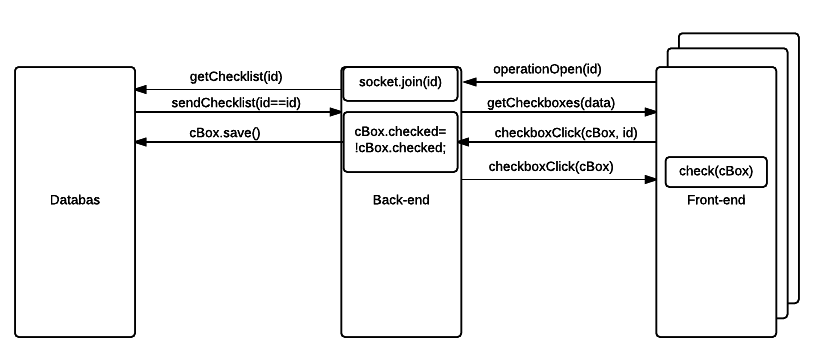
\includegraphics[scale=0.5]{checklistdiagram}\\

När två klienter går in på en operation och en klient checkar en checkruta för första gången tar det strax under en sekund innan checkrutan checkas för den andra klienten. Därefter när någon klient checkar en checkruta så kan jag inte se någon fördröjning alls från det att en klient checkar en checkruta och en annan klient får den checkrutan checkad.\\

Kunden har prövat att ha flera personer inne på samma plocklista samtidigt och checka av olika artiklar. Kunden tyckte att det fungerade bra och påpekade inte någon fördröjning. \\

All information som krävs för plocklistorna fick plats med mycket mellanrum och upplevs därav inte som plottrigt.

\subsection{Diskussion}
\subsubsection{Resultat}
Eftersom jag endast skickar data om vilken checkruta som ska checkas till de klienter som är inne på den operation som checkrutan blev checkad på så uppdateras checkningar snabbare än att göra den enkla lösningen att bara skicka datat till alla anslutna klienter. Att det tar nästan en sekund för en checkning att uppdateras på andra klienter för första gången är långsammare än förväntat. Men eftersom det endast gäller just första artikeln och att kunden har testat checkning med flera personer samtidig utan att märka några problem så verkar detta inte vara något praktiskt problem. Att en checkning sedan kan uppdateras nästan helt utan fördrdröjning var bättre än vad jag hade förväntat mig.

\subsubsection{Metod}
Den metod jag använde mig av fungerade bra, men jag tror att jag skulle kunnat komma fram till samma resultat snabbare genom att göra kortare funktioner och vettigare namn redan från början istället för att göra något som funkar så snabbt som möjligt och sedan refaktorisera. För nu blev det väldigt förvirrande kod från början och jag var tvungen att sitta och tänka på vad kod jag skrivit faktiskt gjorde. Men att skissa olika förslag på ett papper först tror jag var en väldigt bra idé, det gjorde att jag fick några möjliga lösningar och sedan kunde jag överväga fördelar och nackdelar med de olika lösningarna för att sedan välja den som verkade bäst. \\

Att jag började med att implementera plocklistan och inte förän den var klar implementera förberedelselistan tror jag också var en bra idé. Jag kunde då till en början fokusera på en typ av checklista och se till att få den att fungera bra. Sedan när förberedelselistan skulle implementeras så kunde jag återanvända väldigt mycket av den kod som jag skrivit till plocklistan.
\pagebreak

\subsection{Slutsatser}
All nödvändig information i plocklistorna fick plats med bra marginal, därav anser jag att svaret på min första frågeställning är: Ja! \\

Jag har lyckats implementera checkning av både plocklistor och förberedelselistor med ungefär samma kod. Checkningen uppdateras för alla klienter som är inne i samma operationsförberedelse. Det är nästan en sekunds fördröjning när en person checkar den första checkrutan i en checklista tills dess att de andra anslutna klienterna får den checkrutan checkad. Efter det att den första rutan är checkad så uppdateras checkningar utan märkbar fördröjning till de andra anslutna klienterna. Därav anser jag att svaret på min andra frågeställning är: Ja!\\

Eftersom kunden har prövat checkningen av cheklistor med flera personer samtidigt och de tyckte att den fungerade bra som helhet så anser jag att syftet med denna del av projektet är upplevt.

\subsection{Referenser}
\vspace{-9mm}
\begin{thebibliography}{9}
\bibitem{websocketbook} Wang Vanessa, Salim Frank, Moskovits Peter; The Definitive Guide to HTML5 WebSocket; New York City APress, 2013.
\bibitem{websocketreport} http://www.scirp.org/journal/PaperInformation.aspx?PaperID=25428
\end{thebibliography}
\newpage
\section{Vidareutveckling av applikation för Region Östergötland - Albert Karlsson}
\subsection{Inledning}
Denna del i rapporten behandlar vad som ska utredas och varför.
\subsubsection{Syfte}
Syftet med denna enskilda utredningen är att underlätta för fortsatt utveckling av webbapplikationen som projektgruppen har skapat. Alla delar i applikationen får inte användas i Region Östergötlands intranät, vilket leder till att en del måste bytas ut.
\subsubsection{Frågeställning}
\begin{itemize}
\item Vad används Keystone till i applikationen?
\item Vad behövs för att ersätta Keystone?
\item Vad behöver ändras för att byta ut databasen från MongoDB till MSSQL?
\item Vilka moduler eller bibliotek i applikationen kräver en licens för kommersiell användning?

\end{itemize}
\subsubsection{Avgränsningar}
Denna rapport gäller endast för vidareutveckling för användning av Region Östergötland. Andra användare kan ha andra krav på applikationen som leder till att denna rapport är ofullständig eller felaktig. 
\subsection{Bakgrund}
Region Östergötland ska ta över arbetet med utvecklingen av webbapplikationen efter att projektgruppen slutfört sitt arbete. För att applikationen ska kunna tas i bruk på riktigt så måste databasen bytas ut till MSSQL då Region Östergötland inte tillåter MongoDB på sina servrar. Då utvecklingen av applikationen har fortgått har Keystone fått en mindre och mindre roll i applikationen. En av Keystones största fördelar är dess enkla och smidiga administratörssystem. Detta används inte alls i applikationen längre och då databsen ska bytas till en annan typ försvinner också en annan stor del av Keystone. Detta ledde till tankar om att Keystone kanske skulle kunna bytas ut mot egenskriven kod eller mindre och mer lättförståliga moduler utan jättemycket arbete.
\subsection{Teori}
En beskrivning och förklaring för många av modulerna som kommer tas upp finns att läsa i avsnitt 3.
\subsubsection{MSSQL}


\subsection{Metod}
För att få en bättre förståelse för Keystones roll i applikationen så kommer först och främst Keystones tekniska dokumentation läsas. 
\subsection{Resultat}
\subsection{Diskussion}
\subsubsection{Resultat}
\subsubsection{Metod}
\subsection{Slutsatser}
\subsection{Referenser}
\vspace{-9mm}
\begin{thebibliography}{9}

\end{thebibliography}



\end{document}
